\documentclass{article}



\usepackage{arxiv}

\usepackage[utf8]{inputenc} % allow utf-8 input
\usepackage[T1]{fontenc}    % use 8-bit T1 fonts
%\usepackage{hyperref}       % hyperlinks
\usepackage{url}            % simple URL typesetting
\usepackage{booktabs}       % professional-quality tables
\usepackage{amsfonts}       % blackboard math symbols
\usepackage{nicefrac}       % compact symbols for 1/2, etc.
\usepackage{microtype}      % microtypography
\usepackage{lipsum}		% Can be removed after putting your text content
\usepackage{graphicx}
\usepackage[numbers]{natbib}
\bibliographystyle{unsrt}

\usepackage{doi}




%\date{September 9, 1985}	% Here you can change the date presented in the paper title
%\date{} 					% Or removing it

\author{ \hspace{1mm}Quentin Duchemin \\
	Swiss Data Science Center\\ EPFL \& ETH Zürich\\ Switzerland\\
	\texttt{quentin.duchemin@epfl.ch} \\
	%% examples of more authors
	\And
	\hspace{1mm}Guillaume Obozinski \\
	Swiss Data Science Center\\ EPFL \& ETH Zürich\\ Switzerland\\
	\texttt{guillaume.obozinski@epfl.ch} 
}

% Uncomment to remove the date
%\date{}



% Useful packages
\usepackage{amsmath}
\usepackage{amsfonts}
\usepackage{graphicx}
\usepackage{multirow}
\usepackage{array}
\newcolumntype{C}[1]{>{\centering\arraybackslash}m{#1}}
\newcolumntype{L}[1]{>{\arraybackslash}m{#1}}

\usepackage{dsfont}
\usepackage{makecell}
\usepackage{comment}
\usepackage{multicol}
\usepackage{diagbox}
\newcommand{\tred}[1]{\textcolor{red}{#1}}

\title{Efficient distributional regression trees learning algorithms for calibrated non-parametric probabilistic forecasts}

% Diagram
\usepackage{tikz}
\newcommand*\circled[1]{\tikz[baseline=(char.base)]{\node[shape=circle,draw,inner sep=2pt] (char) {#1};}}

\usetikzlibrary{positioning}
\usetikzlibrary{matrix,positioning,arrows.meta,arrows,trees}
\tikzset{
mymat/.style={
  matrix of math nodes,
  text height=2.5ex,
  text depth=0.75ex,
  text width=3.25ex,
  align=center,
  column sep=-\pgflinewidth
  },
mymats/.style={
  mymat,
  nodes={draw,fill=#1}
  }  
}

\usepackage{mathtools}
\DeclarePairedDelimiter\floor{\lfloor}{\rfloor}
\DeclarePairedDelimiter\ceil{\lceil}{\rceil}
\usepackage{subcaption}




\newcommand\blfootnote[1]{%
  \begingroup
  \renewcommand\thefootnote{}\footnote{#1}%
  \addtocounter{footnote}{-1}%
  \endgroup
}

\usepackage{twoopt}
\usetikzlibrary{fit}
\newcommand\tikzmark[1]{%
  \tikz[remember picture,overlay]\node[inner xsep=0pt] (#1) {};}
\newcommandtwoopt\Textbox[5][2.5cm][2cm]{%
\begin{tikzpicture}[remember picture,overlay]
  \coordinate (aux) at ([xshift=#1]#4);
  \node[inner ysep=5pt,yshift=0.ex,draw=red,thick,
    fit=(#3) (aux),baseline] 
    (box) {};
  \node[text width=#2,anchor=north east,
    font=\sffamily\footnotesize,align=right] 
    at (box.north east) {#5};
\end{tikzpicture}%
}


\usepackage{amsthm}
\newtheorem{theorem}{Theorem}
\newtheorem{lemma}{Lemma}
\newtheorem{definition}{Definition}
\date{}

\newdimen\nodeDist
\nodeDist=35mm

\usepackage{algorithm}
\usepackage{algpseudocode}

%\usepackage[colorlinks=true, allcolors=blue]{hyperref}

% Uncomment to override  the `A preprint' in the header
\renewcommand{\headeright}{}
\renewcommand{\undertitle}{}
%\renewcommand{\shorttitle}{\textit{arXiv} Template}

%%% Add PDF metadata to help others organize their library
%%% Once the PDF is generated, you can check the metadata with
%%% $ pdfinfo template.pdf
\hypersetup{
pdftitle={A template for the arxiv style},
pdfsubject={q-bio.NC, q-bio.QM},
pdfauthor={David S.~Hippocampus, Elias D.~Striatum},
pdfkeywords={First keyword, Second keyword, More},
}

\begin{document}
\maketitle

\begin{abstract}
    The perspective of developing trustworthy AI for critical applications in science and engineering requires machine learning techniques that are capable of estimating their \emph{own uncertainty}. 
    In the context of regression, instead of estimating a conditional mean, this can be achieved by producing a predictive interval for the output, or to even learn a model of the conditional probability $p(y|x)$ of an output $y$ given input features $x$. 
    While this can be done under parametric assumptions with, e.g. generalized linear model, these are typically too strong, and non-parametric models offer flexible alternatives. In particular, for scalar outputs, learning directly a model of the \emph{conditional cumulative distribution function} of $y$ given $x$ can lead to more precise probabilistic estimates, and the use of proper scoring rules such as the \emph{weighted interval score} (WIS) and the \emph{continuous ranked probability score} (CRPS) lead to better coverage and calibration properties.
    
    This paper introduces novel algorithms for learning probabilistic regression trees for the WIS or CRPS loss functions.
    %{\color{red}The sum of pinball losses and CRPS are attractive scoring rules in that they address calibration as well as sharpness.}
    %The sum of pinball losses and CRPS are both widely used metrics in quantile regression and probabilistic forecasting, providing robust measures of uncertainty in predictive models. 
    These algorithms are made computationally efficient thanks to an appropriate use of known data structures - namely \emph{min-max heaps, weight-balanced binary trees} and \emph{Fenwick trees}.
    
    Through numerical experiments, we demonstrate that the performance of our methods is competitive with alternative approaches. Additionally, our methods benefit from the inherent interpretability and explainability of trees. As a by-product, we show how our trees can be used in the context of conformal prediction and explain why they are particularly well-suited for achieving \emph{group-conditional coverage guarantees}.
\end{abstract}


% keywords can be removed
%\keywords{First keyword \and Second keyword \and More}
\section{Introduction}

Unlike standard regression methods which target the conditional mean of the response to explanatory variables, distributional regression aims at estimating the entire conditional distribution of the outcome. Distributional regression is becoming more and more popular since understanding variability and uncertainty is crucial in fields like econometrics, climatology, and biostatistics. \cite{rigby2005} laid foundational work with their generalized additive models for location, scale, and shape, in which a parametric distribution is assumed for the response variable but the parameters of this distribution can vary according to explanatory variables using linear, nonlinear or smooth functions. Another line of work relies on density estimation techniques to learn the conditional distributions with methods ranging from mixture models \cite{grun2007fitting} to Bayesian ones \cite{dunson2007bayesian}. More recently, the deep learning area gave birth to generative models achieving remarkable results, especially in the field of imaging \cite{rombach2022high}. These generative models aim at learning to sample from the training data distribution via a transformation of a
simple distribution. One can mention normalizing flows \cite{kobyzev2020normalizing} or diffusion models \cite{ho2020denoising}. These methods have been widely applied to images and text, but recent works \cite{shen2024} adapt these methods to classical regression. We refer to a recent review of distributional regression approaches in \cite{kneib2023}.


While distributional regression provides a comprehensive view of the response distribution, there are cases where practitioners are interested in specific aspects of this distribution, rather than the entire probability landscape. For instance, understanding the behavior of a response variable at its extremes or at specific percentiles can be crucial for applications such as risk assessment or resource allocation. This is where quantile regression \cite{koenker1978regression,regression2017handbook} becomes a powerful complementary tool. Quantile regression has become a standard technique and is usually achieved by minimizing the so-called pinball loss. The pinball loss $\ell_{\tau}$ for the quantile of level $\tau \in (0,1)$ is defined by
\[\ell_{\tau}(\xi) = (\tau- \mathds 1_{\xi <0})\xi,\quad \xi \in \mathds R\]and is such that
\[q_{\tau}(x) \in {\arg \min}_{q \in \mathds R} \mathds E_P[ \ell_{\tau} (Y -q) \mid X=x],\]
where $q_{\tau}(x)$ is the quantile of level $\tau$ of the distribution of $Y$ conditional on $X=x$. While the pinball loss is not differentiable at zero, optimization can still be performed using subgradient methods or by employing a smoothed approximation, such as the Huber loss for the median. This approach enables the use of standard regression models to estimate specific conditional quantiles of interest. Notable examples include the use of neural networks \cite{CANNON20111277}, kernel methods \cite{Takeuchi20061231}, Gaussian processes \cite{Abeywardana20151686} or splines \cite{thompson2010bayesian}. We refer to the survey paper \cite{torossian2020} for a more exhaustive list of quantile regression methods. 


Simultaneous multiple quantile regression provides a natural bridge between full distributional regression and single quantile regression. Estimating a large set of quantiles rather than a single one can be important in various applications such as decision making \cite{Hamilton1999}, personalized health \cite{kulasekera2022quantiles} or finance \cite{Engle2004} where professionals often need to understand the potential losses or gains at various quantiles to assess the risk of different investments or portfolios. A straightforward approach to multiple quantile regression involves fitting separate models for each quantile of interest. However, this method can be suboptimal in practice, as it fails to leverage the shared information between the models, potentially leading to poorer performance. Additionally, it may result in the undesirable phenomenon of quantile crossing, where estimated quantiles are inconsistent, namely when higher quantiles are lower than lower quantiles. To address these issues, regularized approaches \cite{ZOU20085296} or constrained methods \cite{liu2009stepwise} have been proposed to couple different quantile models. To improve computational efficiency, a promising strategy is to optimize the sum of pinball losses across multiple quantiles in a single model \cite{juban2016multiple}, rather than fitting separate models for each quantile. The sum of pinball losses is known as the weighted interval score (WIS) in the probabilistic forecasting community \cite{WIS}. Given $M$ quantile levels $0<\tau_1<\dots <\tau_M<1/2$, the WIS loss is defined by:
\[\ell_{WIS(\tau_{1:M})}(\{q_{\tau_m}\}_{m=1}^{2M+1}, y)=\frac{2}{2M+1} \sum_{m=1}^{2M+1} \ell_{\tau_m}(y-q_{\tau_m}),\]
where $\tau_{M+1}=1/2$ and where $\tau_{M+2}=1-\tau_{M}$, ..., $\tau_{2M+1}=1-\tau_{1}$. The WIS is primarily a loss function on quantiles, but can actually be interpreted as a loss function over a cumulative distribution function~$F$ writing
\[\ell_{WIS(\tau_{1:M})}(F, y)=\frac{2}{2M+1} \sum_{m=1}^{2M+1} \ell_{\tau_m}(y-F^{-1}(\tau_m)).\]
By increasing the number of quantiles considered, one intuitively expects the WIS loss to be sensitive to any change in the cumulative distribution function $F$.  This intuition can be formalized, as shown in~\cite{Brehmer_2021}, by proving that the WIS loss asymptotically converges to the continuous ranked probability score (CRPS) as $M\to \infty$:
\[\mathrm{CRPS}(F,y) := \int_{-\infty}^{+\infty} \big( F(s) - \mathds 1_{s\geq y}\big)^2 ds.\]
The CRPS is a metric designed to evaluate the accuracy of probabilistic predictions. This convergence bridges the gap between quantile-based evaluation and full distributional assessment.




While the CRPS and WIS losses are appealing for training better-calibrated probabilistic forecasters, their adoption in practice remains limited due to several challenges. Firstly, optimizing the risk associated to the CRPS loss can be computationally challenging since explicit solutions are only
available for limited parametric cases \cite{jordan2017evaluating} and gradients of the CRPS might be tractable under some strong assumption on the data distribution \cite{camporeale2021accrue}. Secondly, most existing methods for minimizing the risk associated to the WIS loss require either adding constraints during training or implementing post-processing adjustments to enforce non-crossing quantiles. These additional procedures not only complicate the optimization process but might also negatively impact overall model performance. Thirdly, and perhaps most critically, many of the recent deep learning-based methods for distributional learning, while powerful, suffer from a lack of interpretability. This is a significant drawback in high-stakes applications, such as the medical field, where understanding model decisions is crucial for trust and accountability. There is, therefore, a growing need for interpretable models that can optimize CRPS or WIS losses while maintaining strong predictive performance and computational efficiency.


Among interpretable models, one of the most popular is regression trees. This can be attributed to their intuitive representation of decision-making processes, which appeals to both experts and non-experts. Additionally, their versatility in handling diverse data types renders them applicable from finance to healthcare, image recognition, or natural language processing. The construction of decision trees entails an iterative process of selecting features to split the dataset, guided by an entropy to quantify the impurity or disorder within nodes. At each node, the algorithm assesses potential splitting thresholds for each feature, choosing the one that minimizes overall impurity. The choice of splitting criteria, namely the choice of the impurity measure, is pivotal in optimizing the tree's ability to capture patterns and make accurate predictions. Most common impurity measures can be expressed as the empirical risk of a corresponding loss function $\ell$, for the optimal value of leaf parameters. These impurity measures can therefore be seen as a generalized form of entropy $H_{\ell}$ associated with the loss function $\ell$,
\begin{equation} \label{eq:entropy_loss}\mathbb H_{\ell}( P) := \inf_{a} \mathbb E_{P}[\ell(a,Y)].\end{equation}
This connection is well-known in the literature \cite[Eq.(2.14)]{degroot62},\cite{grunwald, Aolin}. The entropy associated with a specific loss function is also referred to as the generalized entropy or the Bayes risk \cite{Aolin,bao2021fenchel}. In both classification and regression settings, the range of entropies employed for training decision trees remains relatively limited. In binary classification, the usual choices for entropy include the Gini entropy, the Shannon entropy, or the 0-1 entropy (cf. \cite{generalizedentropy}) corresponding respectively to the squared loss, the log loss and the 0-1 loss. For regression, common practice involves opting for a splitting criterion based on the squared loss or the absolute error.

%Choosing the right entropy is important when training decision trees. The choice of entropy directly influences the decision tree's ability to effectively capture the desired patterns and thus to make accurate predictions. 
In this work, we present two novel algorithms for efficiently training distributional regression trees for the WIS loss and the CRPS loss. 

% Quantifying uncertainty with regression trees
\paragraph{Related work.}
As far as we know, there are two ways to learn a conditional quantile model using regression trees in the current literature:
\begin{itemize}
\item Either one uses the so-called Quantile Regression Forest method \cite{meinshausen2006quantile}. %In this case, several trees are trained using the squared loss and thus target the conditional mean of the data distribution. To obtain an estimate of the conditional quantile or level $\tau$ for a test sample $x$, one drops $x$ down all the trees and collects all the training output values $y_i$ found in the leaves where we end. This process enables the construction of an estimate of the conditional distribution of the response variable, from which one can query the quantile of interest. 
This method, by using the squared loss, benefits from well-established and optimized packages for training regression trees. Additionally, these trees can be used to estimate quantiles of any level with the resulting quantiles guaranteed to be non-crossing (cf. \cite[Section 6]{romano2019conformalized}). However, a key drawback is that the splitting criterion used to construct the tree is well adapted to capture the fluctuations of the conditional mean but not the conditional quantiles of interest, which potentially decreases statistical efficiency.    %This approach presents two main drawbacks. Firstly, it is computationally intensive, necessitating the training of a large set of trees for accurate quantile estimation. Secondly, each tree aims to estimate the conditional mean (rather than the conditional quantiles of interest), potentially sacrificing statistical efficiency. 
\item \cite{bhat2015} considers the problem of learning a single conditional quantile model using a single quantile regression trees trained with the quantile loss function, also known as the pinball loss. 
The entropy associated to the pinball loss is
\begin{align*}\mathbb H_{\ell_{\tau}}( P) &=  \min_{q \in \mathds R} \mathds E_P[ \ell_{\tau} (Y -q)]\\
&= (1-\tau) \mathds E_P[(q-Y)_+] + \tau \mathds E_P[(Y-q)_+],
\end{align*}
where for any real number $x$, $(x)_+=\max(x,0)$.
In the empirical setting where we have observations $\textbf y=\{ y_i \}_{i=1}^n$ sampled from $P$, the empirical entropy is 
\begin{align}\label{eq:empi_pinball} H_{\ell_{\tau}}(\textbf y) :=\min_{q \in \mathds R} \frac{1}{n}\sum_{i=1}^n \ell_{\tau} (y_i -q)=\frac{1}{n}\sum_{i=1}^n \ell_{\tau} (y_i -\hat q_{\tau}),
%&=\frac1n(1-\tau) \sum_{i\leq [\tau n]}(y_{([\tau n])}-y_{(i)}) + \frac1n\tau \sum_{i>[\tau n]}(y_{(i)} -y_{([\tau n])})\\
%= y_{(\floor{\tau n})}\big( \frac{\floor{\tau n}}{n}-\tau\big) + \frac{\tau}{n}\sum_{i=1}^n y_i - \frac1n \sum_{i\leq \floor{\tau n}} y_{(i)},\label{eq:pinball_entropy}
\end{align}
where $\hat q_{\tau} = y_{(\lceil\tau n\rceil)}$ is the empirical quantile of level $\tau$ of the sequence $\textbf y=(y_i)_{i=1}^n$. The tree is then trained using the standard CART algorithm \cite{breiman2017classification} with the entropy from Eq.\eqref{eq:empi_pinball}: at each node, the data is split by selecting the feature and the threshold that minimize the entropy within the resulting subsets. This process iteratively creates nodes that represent the most homogeneous possible groups by reducing overall entropy.
The procedure to find the data split maximizing the information gain defined with the entropy from Eq.\eqref{eq:empi_pinball} at a given node of the tree with $n$ samples and $d$ features has a time complexity of order $\mathcal O(dn\log n)$ (cf. \cite{bhat2015}). 
\end{itemize}
In this paper, we complement the work of \cite{bhat2015} by presenting two efficient algorithms to learn distributional regression trees for the WIS and CRPS losses.

\paragraph{Outline.}

In this work, we first introduce two novel algorithms to learn distributional regression trees (Sec.~\ref{sec:RT}): the first minimizes the empirical entropy associated to the WIS loss, which we call Pinball Multiple Quantiles Regression Trees (PMQRT); the second algorithm learns distributional regression trees (CRPS-RT) for the CRPS loss. To improve the latter algorithm, we propose to use an unbiased estimate of the CRPS risk using leave-one-out without additional computational cost (Sec.~\ref{sec:CRPS-LOO}). Detailed descriptions of the algorithms can be found in Section~\ref{apdx:algos}. In Section~\ref{sec:expes}, we conduct an empirical evaluation of our algorithms through a series of experiments. We demonstrate the scalability of the proposed algorithms and that by using a forest of CRPS-RT (CRPS-RF), we can develop a non-parametric method for learning conditional distribution functions that rivals existing approaches. 





\section{Learning distributional regression trees}
\label{sec:RT}
%\tred{An introduction to this section is missing here. Unless I missed it, the main proposal that we make which is to learn a tree which has \emph{common} splits for all quantiles or for the whole conditional distribution, has not really been introduced yet or been emphasized clearly until now. Even if it has been mentioned, the introduction of this section would be the perfect place to explain that, because this is the way to explain where we are going from now on. If you think about it the whole difficult of this section is to construct algorithms to determine these best commmon splits...}

This section introduces algorithms designed to construct regression trees with common splits for modeling multiple quantiles or the entire conditional distribution. Unlike traditional approaches that treat different quantiles independently, our methods seek to identify shared split points to improve interpretability and computational efficiency. We propose two tree-learning algorithms tailored to distinct loss functions: one for the WIS and another for the CRPS. The following subsections outline these methods and address the challenges inherent in optimizing these distinct objectives.

\subsection{Notations}
To consider possible splits according to one variable, we will have to sort the data according its values, consider the $s$ points before a split, and compute an empirical quantile (which is an order statistic) of the corresponding labels. This motivates the introduction of the following notations: Let us consider an arbitrary sequence $\textbf a = (a_1,\dots,a_n)$ of real values of size $n$. For any $s\in[n]$, we denote by $\textbf a^{(s)}:=(a_1,\dots,a_s)$ the prefix sequence of $\textbf a$. For any $s\in [n]$, $a_{(s)}$ corresponds to the $s$-th largest value of the sequence $\textbf a$, while  for any $i \in [s]$, $a^{(s)}_{(i)}$ refers to the $i$-th largest value of the prefix sequence $\textbf a^{(s)}$. %In this section, we assume that the data consists in i.i.d.\ samples $\{(\textbf x_i,y_i)\}_{i=1}^n$ drawn from a common distribution $P$ on $\mathbb R^d \times \mathbb R$.

\subsection{Pinball multi-quantile regression tree}

\begin{comment}\tred{This section starts rather abruptly with a technical description of the algorithm of~\cite{bhat2015}, without a clear connection to the title and without telling the reader where we are going with this... I would suggest to proceed as follows:
\begin{enumerate}
\item First explain that, while we could learn separate trees for each quantile, we propose to design a learning algorithm that learns a tree producing at each leaf all conditional quantiles estimates, and which most importantly uses common split for all quantiles based on $\ell_{\tau_1,\ldots,\tau_m}$ which I would define here (see further for now). I would have already in this section the explanation that the problem is separable in each leaf, but that we need to consider all quantile losses to determine the splits, which shoud be determined according to the entropy. I would explain that this is similar to ~\cite{bhat2015} but with multiple quantiles at the same time
\item Then I would have a subsection entitled "Efficient pinball loss node splitting with max heaps" which is strictly dedicated to summarizing what ~\cite{bhat2015} does. And in fact maybe this is where the Notation section should be inserted.
\item Third, I would have another subsection in which you explain how to generalize their algorithm in a non-naive way.
\end{enumerate}
}
\end{comment}
%{\color{blue} $\rightarrow$ Regarding the paragraph with notations, I am not sure since those notations are also useful for the CRPS section.}
%For multiple quantile regression trees, a naive approach would consist in exploiting a method similar to the case of a single quantile for each level of interest. 

\paragraph{Extracting multiple quantiles from a single tree.} 
When estimating multiple quantiles at different levels, one option is to use Quantile Regression Forests (QRF), where the set of trained trees can be queried to estimate any quantile. However, as noted earlier, these trees are learned using the square loss and aim to predict the conditional mean of the data distribution, which may result in suboptimal estimates for the quantiles.

A simple alternative consists of relying on a set of trees, each targeting a specific quantile level \(\tau\) and learned following the method from~\cite{bhat2015} to minimize the entropy associated with the pinball loss \(\ell_{\tau}\). This approach has two main limitations. First, we lose the guarantee of non-crossing quantiles, which holds in the QRF method. Second, each learned tree forms its own partition of the feature space based on the quantile level it is targeting. This not only hampers the application of these trees for tasks such as group conformal prediction (cf. Section~\ref{sec:group_conformel}), but it may also lead to reduced statistical efficiency due to the lack of a unified feature space partitioning and the potential increase in the variance of the quantile estimates. 

To bypass these limitations, we present an approach that takes the best of the ones above-mentioned. We propose learning a tree that produces all conditional quantiles estimates in each leaf and that most importantly relies on a common split for all quantiles considering the sum of pinball losses $\ell_{\tau_1,\ldots,\tau_m}$ defined for any ${\boldsymbol \tau},\mathbf{q} \in \mathbb{R}^M$ as \[\ell_{\tau_1,\ldots,\tau_m}(\mathbf{q},y):=\sum_{m=1}^M \ell_{\tau_m}(y-q_m).\]
The multi-dimensional optimization problem over $\mathbf{q}\in\mathbb R^M$ that defines the empirical entropy associated with~$\ell_{\tau_1,\ldots,\tau_m}$ is separable, which leads to \begin{equation} \label{eq:multi_entropy}H_{\ell_{\tau_1,\ldots,\tau_m}}(\mathbf{y})=\sum_{m=1}^M H_{\ell_{\tau_m}}(\mathbf{y}).\end{equation}
Relying on the CART algorithm, training a regression tree considering the loss $\ell_{\tau_1,\ldots,\tau_m}$ requires to compute the entropies $H_{\ell_{\tau_1,\ldots,\tau_m}}(\textbf y^{(s)})$ associated to any prefix sequence $\textbf y^{(s)}:= (y_1,\dots, y_s)$ from a given sequence of values $\textbf y=(y_1,\dots,y_n)$. We end up with a problem similar to~\cite{bhat2015} but with multiple quantiles at the same time.

\paragraph{Efficient pinball loss node splitting with max heaps.} 
The algorithm proposed in \cite{bhat2015} for learning a quantile regression tree that minimizes the empirical entropy associated with a single pinball loss $\ell_{\tau}$ uses two heaps (cf. \cite{halim2013competitive}). At a given node in the tree, with data $\{(\textbf{x}_i, y_i)\}_{i=1}^n$, the goal is to find the threshold that provides the best information gain using the entropy from Eq.\eqref{eq:empi_pinball} for each feature $j$. Assuming without loss of generality that $[\textbf{x}_{1}]_j \leq \dots \leq [\textbf{x}_{n}]_j$ for some feature $j$, identifying the optimal threshold reduces to computing the entropies for all prefix and suffix sequences of $\textbf{y}$. Since the suffix sequences of $\textbf{y}$ correspond to prefix sequences of $(y_{(n)}, \dots, y_{(1)})$, it's sufficient to explain how \cite{bhat2015} computes efficiently the entropies of the sequences $\textbf{y}^{(s)}$ for all $s \in [n]$. As shown in \cite[Sec.III.B]{bhat2015}, the entropy $H_{\ell_{\tau}}(\textbf{a})$ for any nondecreasing sequence $\textbf{a}$ of length $s$ can be computed in $\mathcal{O}(1)$ time using $a_{\lceil\tau(s-1)\rceil}$, $a_{\lceil\tau s\rceil}$, $\sum_{i=1}^{\lceil\tau(s-1)\rceil} a_{(i)}$, and $\sum_{i=1}^s a_i$. The authors show that these quantities can be efficiently tracked by initializing two empty heaps - one max-heap $\mathcal H_{low}$ and one min-heap $\mathcal H_{high}$ - and by sequentially adding elements $y_s$ from $s=1$ to $n$ to them. At each step $s$, the update of the two heaps ensures that $\mathcal H_{low}$ contains all elements $(y_{(1)}, \dots, y_{(\lceil\tau(s-1)\rceil)})$ and $\mathcal H_{high}$ contains all elements $(y_{(\lceil\tau s\rceil)}, \dots, y_{(s)})$. Querying the maximum value in $\mathcal H_{low}$ and the minimum value in $\mathcal H_{high}$ can be done in constant time while the heaps update require $\mathcal{O}(\log(s))$ time.

From Eq.~\eqref{eq:multi_entropy}, the empirical entropy of a sum of pinball losses \(\ell_{\tau_1, \dots, \tau_M}\) is the sum of the empirical entropies for each individual pinball loss. As a consequence, a straightforward approach to estimate quantiles at multiple levels using a single tree is to apply the method from \cite{bhat2015} independently for each quantile level. However, this brute-force approach incurs a space complexity of \(\mathcal{O}(Mn)\), making it inefficient as the number of quantile levels \(M\) increases.

To address this limitation, we propose a new algorithm whose space complexity remains of the order of the size of the dataset, regardless of the number of estimated quantiles. 

\paragraph{Efficient pinball multi-quantile loss node splitting with a set of min-max heaps.} 

%Relying on the CART algorithm, training such a tree requires to compute the entropies \begin{equation*} \label{eq:multi_entropy}  H_{\sum_{m=1}^M\ell_{\tau_m}}(\textbf y^{(s)})=\min_{q_{\tau_1},\dots,q_{\tau_M} \in \mathds R} \frac{1}{nM}\sum_{m=1}^M\sum_{i=1}^n \ell_{\tau_m} (y_i -q_{\tau_m}).\end{equation*}
%=\sum_{m=1}^M \mathcal H_{\ell_{\tau_m}}(\textbf y^{(s)}),\] associated to any prefix sequence $\textbf y^{(s)}:= (y_1,\dots, y_s)$ from a given sequence of values $\textbf y=(y_1,\dots,y_n)$. One can notice that Eq.\eqref{eq:multi_entropy} can be written as $M$ independent optimization problems, each one with a closed form solution obtained using $\hat q_{\tau_m}$. 
Using the decomposition Eq.~\eqref{eq:multi_entropy}, one can deduce from~\cite{bhat2015} that the empirical entropy $H_{\ell_{\tau_1,\ldots,\tau_m}}(\textbf y^{(s)})$ of any prefix sequence $\textbf y^{(s)}$ can be obtained by keeping track of $i)$ the empirical quantiles $\widehat q_{\tau_1},\dots,\widehat q_{\tau_M}$ of level $\tau_1,\dots,\tau_M$ of $\textbf y^{(s)}$ and $ii)$ of the cumulative sums $\left( \sum_{i\leq \ceil{\tau_m s}}y^{(s)}_{(i)}\right)_{m=1}^M$ and $\sum_{i\leq s}y^{(s)}_{(i)}$. We propose an efficient algorithm to keep track of these quantities relying on $M+1$ min-max heaps: $\mathcal H_{1},\dots,\mathcal H_{M}, \mathcal H_{M+1}$. Let us recall that a min-max heap is a variant of a binary heap allowing for constant-time access to both the minimum and maximum elements. On even levels, the heap adheres to min-heap properties, while odd levels follow max-heap properties. This ensures that the root always holds the minimum, and its children represent the maximum elements. Insertions and deletions have logarithmic time complexity, providing a balance between efficient extremal element access and effective heap modification.
As for standard regression trees, we increase the index $s$ from 1 to $n$ to cover all the prefix sequences $\textbf y^{(s)}$ of interest to determine the position of the split at the current node. The $M+1$ min-max heaps are updated at each iteration $s$ to ensure that $\mathcal H_{1}$ contains all the elements $\{y^{(s)}_{(1)},\dots y^{(s)}_{(\ceil{\tau_1 s})} \}$, $\mathcal H_{2}$ contains all the elements $\{y^{(s)}_{(\ceil{\tau_1 s}+1)},\dots y^{(s)}_{(\ceil{\tau_2 s})}\}$, $\dots$ , $\mathcal H_{M}$ contains all the elements $\{y^{(s)}_{(\ceil{\tau_{M-1} s}+1)},\dots y^{(s)}_{(\ceil{\tau_M s})}\}$, and $\mathcal H_{M+1}$ contains all the elements $\{y^{(s)}_{(\ceil{\tau_M s}+1)},\dots y^{(s)}_{(s)}\}$. Querying the quantile of level $\tau_m$ simply involves accessing the maximum of the heap $\mathcal H_m$, or the minimum of the heap $\mathcal H_j$ for $j:=\arg \min \{i >m\mid \mathcal H_i\neq \emptyset\}$ in case $\mathcal H_m$ is empty. Our min-max heap structures are also designed to store the total sums of elements in each heap, facilitating access to cumulative sums of the form $\sum_{i\leq \lceil\tau_m s\rceil}y^{(s)}_{(i)}$ in $\mathcal O(m)$ time by querying the total sums of heaps $\mathcal H_1$ to $\mathcal H_m$. Overall, the worst time complexity for a node split with $n$ data points and $d$ features is $\mathcal O(Md n\log n)$ as illustrated in Table~\ref{tab:time_complexity}. The detailed algorithm can be found in Section~\ref{apdx:regression_tree_multi_quantiles}.

%At each step $s$, we add to the previous prefix sequence $\textbf y^{(s-1)}$ a new element $y_{s}$. To keep track of the quantities $\widehat q_{\tau_1},\dots,\widehat q_{\tau_M}$ and $\left( \sum_{i\leq \ceil{\tau_m s}}y^{(s)}_{(i)}\right)_{m=1}^M$, 





\subsection{CRPS distributional regression tree}
\label{sec:CRPS}

In the previous section, we presented a computationally efficient method for learning a Pinball multi-quantile regression tree. Such a tree has the advantage of leveraging information from different parts of the conditional distribution to build the partition, ensuring non-crossing quantile estimates, and offering a flexible tool for modern uncertainty quantification, ideal for applications such as group conformal methods, see Section~\ref{sec:group_conformel}. However, a Pinball multi-quantile regression tree focuses only on specific quantiles, limiting its ability to represent the full conditional distribution. As a result, it may overlook key aspects of the data distribution, affecting predictive accuracy. Furthermore, certain methods, such as the distributional conformal prediction method proposed in \cite{chernozhukov2021distributional}, require querying quantiles at arbitrary levels, and constraining the model to a fixed set of predefined quantiles may hinder its effectiveness. 

To bypass these limitations, we propose to learn trees that minimize the empirical entropy associated with the Continuous Ranked Probability Score (CRPS), namely \begin{equation}  H_{\mathrm{CRPS}}(\textbf y):=\min_F \frac1n \sum_{i=1}^n \mathrm{CRPS}(F,y_i) = \frac1n \sum_{i=1}^n \mathrm{CRPS}(\widehat F_n,y_i) , \label{eq:CRPS_empirical}\end{equation}
where $\widehat F_n$ is the empirical CDF of the observed data $\textbf y$. The CRPS is a strictly proper scoring rule, as detailed in \cite{gneiting2007strictly}, incentivizing forecasters to provide accurate and well-calibrated uncertainty estimates, making it a valuable tool in probabilistic forecasting evaluations. 

To construct a distributional regression tree based on the generalized entropy induced by the CRPS loss, one must identify the split at a given leaf that results in the largest impurity gain. %This requires evaluating all possible thresholds. 
Given a leaf with data $\left\{(\textbf{x}_i, y_i)\right\}_{i=1}^n$, this process involves computing the entropies for every feature $j$ using every prefix sequence $\textbf{y}^{(s)} = \left\{y_1, \dots, y_s\right\}$ and every suffix sequence $(y_{s+1}, \dots, y_n)$ of the data sequence $\textbf{y}$, assuming for simplicity that $x_{1,j} \leq \dots \leq x_{n,j}$. Relying on the entropy expression from Eq.~\eqref{eq:CRPS_empirical}, this requires constructing the empirical CDFs for all prefix and suffix sequences of $\textbf{y}$ for each feature $j$. This process is computationally intensive: specifically, constructing the empirical CDFs for the prefix sequences of a feature $j$ necessitates sequentially inserting a new element $y_{s+1}$ into the current sorted version of the list $\textbf{y}^{(s)}$, with a time complexity of $\mathcal{O}(s)$. Consequently, the basic construction of a distributional regression tree based on the CRPS loss results in a node split with a time complexity of $\mathcal{O}(d n \log(n) \sum_{i=1}^n s) = \mathcal{O}(d n^3 \log n)$, which is not feasible for practical use.

To efficiently train a tree using the CRPS loss, reducing computations is key. Due to the sequential structure of the computation of entropies associated to prefix (resp. suffix) sequences to perform a node split, one can investigate the possibility to rely on iterative schemes to reduce the computational burden of the algorithm. Theorem~\ref{thm:indu} presents an iterative formula allowing to compute the entropies associated to all prefix sequences for a given feature $j$. Note that a similar formula is directly obtained from Theorem~\ref{thm:indu} for suffix sequences by flipping the sign of each entry of the feature vectors $\left\{\textbf x_i\right\}_{i=1}^n$.


\begin{theorem}
Let us consider a leaf with data $\left\{(\textbf{x}_i, y_i)\right\}_{i=1}^n$ and a given feature $j$. Assume without loss of generality that $x_{1,j} \leq \dots \leq x_{n,j}$ and let us denote by $\textbf y^{(s)}$ the prefix sequence $(y_1,\dots,y_s)$ of size $s$ and $\widehat F_s$ the empirical CDF of $\textbf y ^{(s)}$. Then, the empirical entropies 
\[ H_{\mathrm{CRPS}}(\textbf y^{(s)}):= \frac{1}{s} \sum_{i=1}^s \mathrm{CRPS}(\widehat F_s, y_i),\]
for all $s\in[n]$ can be computed using an iterative scheme. Indeed, we have
\[ H_{\mathrm{CRPS}}(\textbf y^{(s+1)})=\frac{1}{(s+1)^3}\left(s^3 H_{\mathrm{CRPS}}(\textbf y^{(s)}) + h^{(s+1)}\right),\]
with
\begin{align*}
h^{(s+1)}
&=h^{(s)}+s\big[2r_{s+1} -3-s\big] y^{(s+1)}_{(r_{s+1})} + 2 W^{(s+1)}-2S^{(s+1)}-2sS^{(s+1)}_{r_{s+1}-1},
\end{align*}
and where for any $r\in[s]$, 
\[S^{(s)}_r:=\sum_{i=1}^{r}y^{(s)}_{(i)}, \quad W^{(s)}:=\sum_{i=1}^s iy^{(s)}_{(i)} \quad \text{and}\quad S^{(s)}:=S^{(s)}_s.\]
For any $s\in[n-1]$, $r_{s+1}$ is the insertion rank of $y_{s+1}$ within the non-decreasing sorted version of the list $\textbf y^{(s)}$.   
\label{thm:indu}
\end{theorem}

Theorem~\ref{thm:indu} shows that training a distributional regression tree using the CRPS loss is achievable if the insertion ranks \(\big(r_s\big)_{s \in [n]}\) and cumulative sums \(S^{(s)}_{r_s-1}\), \(S^{(s)}\), and \(W^{(s)}\) can be computed efficiently.

For a given feature $j$, the process begins by sorting the list of feature entries $\left\{x_{i,j}\right\}_{i=1}^n$, which requires $\mathcal{O}(n \log n)$ time. Once sorted, the insertion ranks $\big(r_s\big)_{s \in [n]}$ can be pre-computed using a weight-balanced tree \cite{Nievergelt73}. Weight-balanced trees offer logarithmic performance similar to that of red-black and AVL trees but also provide the advantage of indexing elements in logarithmic time. Lemma~\ref{lemma:WB_tree} shows that these ranks can be pre-computed in $\mathcal{O}(n \log n)$ time.


\begin{lemma} \cite[Chapter 10]{mehta2004handbook}
A weight-balanced tree with data $\textbf{y}^{(s)}$ allows inserting a new value $y_{s+1}$ and determining its position in the sorted version of the list $\textbf{y}^{(s)}$ such that the resulting list remains in non-decreasing order, all in $\mathcal O(\log s)$ time.
\label{lemma:WB_tree}
\end{lemma}

Once the ranks $\big(r_s\big)_{s \in [n]}$ are computed, we need to obtain the entropies $ H_{\mathrm{CRPS}}(\textbf y^{(s)})$ for any prefix sequence $\textbf y^{(s)}$ using the iterative scheme presented in Theorem~\ref{thm:indu}. For this, it is sufficient to query efficiently the sums $S^{(s)}_{r_s-1}$, $S^{(s)}$ and $W^{(s)}$. 


\begin{definition}
% Let us denote by $\sigma$ a permutation sorting the list $\textbf y$ in increasing order (i.e. $y_{\sigma(1)}\leq \dots \leq y_{\sigma(n)}$) and let us further define:
% \[p^{(s)}_{i}:= \left\{
%     \begin{array}{ll}
%         \mbox{rank of }y_i \mbox{ when sorting } \textbf y ^{(s)} & \mbox{if } i\leq s \\
%         0 & \mbox{if } i>s
%     \end{array}
% \right..\]
% By construction, we have $r_s=p^{(s)}_s$. 
Let us denote by $\sigma$ a permutation sorting the list $\textbf y$ in non decreasing order (i.e. $y_{\sigma(1)}\leq \dots \leq y_{\sigma(n)}$). We define by $\mathcal F$ a Fenwick tree of size $n$ initialized with $n$ zero values such that at any iteration $s\geq 1$, we add the element $y_s$ at the position $\sigma^{-1}(s)$ in the list represented by the Fenwick tree $\mathcal F$. 
\label{def:fenwick}
\end{definition}
In Definition~\ref{def:fenwick}, we introduce a data structure $\mathcal F$ being a specific instance of a Fenwick tree. A Fenwick tree, as shown in Figure~\ref{fig:fenwick_tree}, makes it possible to query any cumulative sum of a list of values in logarithmic time in the size of the list while adding an element to the tree also has a logarithmic time complexity. By construction at any iteration $s$, $\mathcal F$ is a Fenwick tree for the list $(\mathrm 1_{\sigma(i)\leq s} y_{\sigma(i)} )_{i\in [n]}$.
In Lemma~\ref{lemma:fenwick_tree}, we demonstrate that $\mathcal F$ enables tracking the cumulative sums of the form $S^{(s)}_{r_s-1}$ and $S^{(s)}$ which, as a by product, allows 
 for monitoring $W^{(s)}$ throughout the iterative process. The proof of Lemma~\ref{lemma:fenwick_tree} is provided in Section~\ref{proof:lemma:fenwick_tree}. 

\begin{lemma}
At iteration $s$, the Fenwick tree $\mathcal F$ allows:
\begin{itemize}
    \item calculating $S^{(s)}_{r_s-1}$ and $S^{(s)}$ in $O(\log n)$ time,
    \item inserting a new value in $O(\log n)$ time,
    %\item deleting a value in $O(\log s)$ time,
    \item computing $W^{(s)}$ from $W^{(s-1)}$ in $O(\log n)$ time.
\end{itemize}
\label{lemma:fenwick_tree}
\end{lemma}


\begin{figure}[!ht]
\centering
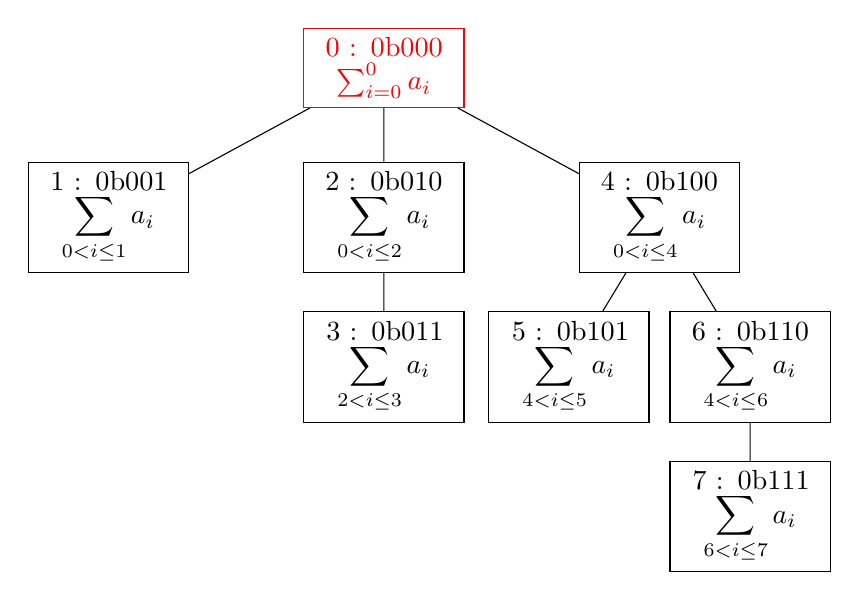
\begin{tikzpicture}[level distance=1.9cm,
level 1/.style={sibling distance=3.5cm},
level 2/.style={sibling distance=2.3cm}]
\tikzstyle{every node}=[rectangle,draw]

\node[text width=1.8cm,align=center] (Root) [red] {0 : 0b000\\ $\sum_{i=0}^0 a_i$}
    child {
    node[text width=1.8cm,align=center] {1 : 0b001 \\ $\displaystyle \sum_{0<i\leq 1} a_i$}
    }
    child {
    node[text width=1.8cm,align=center] {2 : 0b010 \\ $\displaystyle \sum_{0<i\leq 2}  a_i$}
    child { node[text width=1.8cm,align=center] {3 : 0b011 \\ $\displaystyle \sum_{2<i\leq 3}  a_i$} }
    }
    child {
    node[text width=1.8cm,align=center] {4 : 0b100 \\ $\displaystyle \sum_{0<i\leq 4}  a_i$}
    child {  node[text width=1.8cm,align=center] {5 : 0b101 \\ $\displaystyle \sum_{4<i\leq 5}  a_i$} }
    child { node[text width=1.8cm,align=center] {6 : 0b110 \\ $\displaystyle \sum_{4<i\leq 6} a_i$}  
        child {   node[text width=1.8cm,align=center] {7 : 0b111 \\ $\displaystyle \sum_{6<i\leq 7}  a_i$} }
        }
    };
\end{tikzpicture}
 \caption{Fenwick tree for a list $(a_i)_{i\in\{1,\dots,7\}}$ of length $7$. By convention, $a_0=0$. The nodes of the tree are indexed by the natural integers. $0$ is at the root and the children of the root correspond to all integers of the form $2^p$ with $p\in \mathbb{N}.$ More generally, nodes at depth $k$ are the sum of $k$ integers of the form $2^p,$ i.e., they have $k$ non-zero bits in their binary expansion. The parent of node $i$ has the same binary expansion except that the lowest non-zero bit of $i$ is set to $0$ in its parent. If $A_j=\sum_{i=0}^j a_i,$ then the partial sum stored at node $i$ is $A_i-A_{\texttt{pa}(i)},$ where $\texttt{pa}(i)$ is the parent of $i$. }
\label{fig:fenwick_tree}
\end{figure}






In Section~\ref{apdx:crps_induction}, we present in details our algorithm to perform a node split to grow a CRPS-RT. Overall, the computational time required to perform a node split scales as $\mathcal O(dn\log n) $ where $n$ is the number of data points in the node and $d$ is the number of features. The time complexity of the two algorithms presented in this paper are given in Table~\ref{tab:time_complexity}.

\begin{table}[!ht]
\centering
\begin{tabular}{c|C{3cm}||C{3cm}}
\textbf{Algorithm} & Multiple Quantiles Regression Trees & CRPS Regression Tree\\\hline
\textbf{Time complexity} & $\mathcal O(Mdn\log n )$ & $\mathcal O(dn\log n ) $
\end{tabular}
\caption{Worst case time complexity for a specific node split for the different regression trees.}
\label{tab:time_complexity}
\end{table}

\subsection{Unbiased estimate of the entropies using leave-one-out}
\label{sec:CRPS-LOO}


To train PQRTs, PMQRTs or CRPS-RTS, we proposed in the previous sections to rely on the standard CART algorithm \cite{breiman1984classification} which leads to biased estimates of entropies. This bias arises because the same data is used both to estimate parameters (such as empirical quantiles or cumulative distribution functions) and to compute the entropies. By doing so, the empirical entropies computed at any step of the training procedure is a biased estimate of the target entropy. A naive solution to mitigate this issue involves splitting the data into two disjoint sets—one for parameter estimation and the other for entropy evaluation. However, such a data-splitting approach is statistically suboptimal since only part of the data is used at each step. To overcome this limitation, we adopt a leave-one-out (LOO) approach which provides unbiased entropy estimates. The pitfall is that the naive implementation of this method is computationally heavy. Fortunately, we show in Section~\ref{apdx:LOO} that this LOO estimate of the entropy can be obtained at no additional cost for both the CRPS loss and the pinball loss.


% To train PQRTs or PMQRTs, previous works rely on the standard CART algorithm \cite{breiman1984classification} in which the same data is used to estimate the empirical quantiles $q_{\beta}^{j,\rightarrow s},q_{\beta}^{j,\leftarrow s}$ and the entropies $h_{j,s}$ (from Section~\ref{sec:quantile_reg_tree}). By doing so, the empirical entropies computed at any step of the training procedure is a biased estimate of the target entropy. To get an unbiased estimate, we use a LOO estimate of the entropy at a node. The pitfall is that the naive implementation of this method is computationally heavy. Fortunately, we show in Section~\ref{apdx:LOO} that this LOO estimate of the entropy can be obtained at no additional cost.



% Similarly, the algorithm proposed in the previous section to train CRPS-RT uses the same data to estimate the CDFs and the entropies. By doing so, the empirical entropies $  H_{\mathrm{CRPS}}(\textbf a)$ computed at any step of the training procedure is a biased estimate of the target entropy given by $\min_{F} \mathbb E[\mathrm{CRPS}(F,Y)]$. To get an unbiased estimate, one could rely on the standard splitting method that partitions the data into two parts $(\mathcal D_1,\mathcal D_2)$, $\mathcal D_1$ being used to compute the empirical CDF $\widehat F$ and the other used to evaluate the entropy with $\frac{1}{|\mathcal D_2|} \sum_{y\in \mathcal D_2} \mathrm{CRPS}(\widehat F, y)$. Such approach is suboptimal since only part of the data is used to estimate the empirical CDF and to approximate the entropy. To improve statistical efficiency, one would like to avoid such splitting approach while still getting a unbiased estimate of the entropies. One standard way to achieve this goal is to use leave-one-out (LOO). The LOO estimate of the entropy at a node with data $\textbf a$ is unbiased and is given by
% \[ H _{\mathrm{CRPS}}^{\mathrm{LOO}}(\textbf a):=\frac1n \sum_{i=1}^n\mathrm{CRPS}(\widehat F^{-i},a_i),\]
% where $\widehat F^{-i}$ is the empirical CDF obtained from the sequence $(a_1,\dots,a_{i-1},a_{i+1},\dots,a_n)$. The pitfall is that the naive implementation of this method is computationally heavy. Fortunately, we show in Section~\ref{apdx:LOO} that this LOO estimate of the entropy of the sequence $\textbf a$ can be obtained by a simple rescaling of the biased empirical entropy $ H_{\mathrm{CRPS}}(\textbf a)$. 




\section{Experiments}
\label{sec:expes}
\subsection{CDF estimation improvement with an unbiased CRPS risk estimate}
To demonstrate the importance of using LOO for calculating information gain, we consider a simple example where the covariate $X$ is uniformly sampled from the interval $(0, 10)$, and \begin{align} \label{eq:simu_gamma}\tag{Gamma}Y \mid X &\sim \text{Gamma}(\text{shape} = \sqrt{X}, \text{scale} = \min\{\max\{X, 1\}, 6\})
\end{align}
Figure~\ref{fig:simu_LOO} shows the estimated conditional CDFs using a forest of 100 CRPS-RTs, comparing the results with and without LOO used for entropy calculation. On this example, applying LOO produces a significantly better estimate of the conditional CDFs. We perform a similar experiment for PMQRF, demonstrating a significant improvement in quantile estimates achieved through the use of LOO. The results of these simulations are presented in Section~\ref{apdx:LOO}.

\begin{figure*}[!ht]
    \centering
    \begin{subfigure}[t]{0.5\textwidth}
        \centering
        \includegraphics[height=2.2in]{gamma_simu_n600_vr.png}
        \caption{With LOO.}
    \end{subfigure}%
    ~ 
    \begin{subfigure}[t]{0.5\textwidth}
        \centering
        \includegraphics[height=2.2in]{gamma_simu_n600_vr_noLOO.png}
        \caption{Without LOO.}
    \end{subfigure}
    \caption{Estimation of the conditional CDF of y given x with CRPS-RF on a sample of size $n=600$ simulated from the distribution in Eq.\eqref{eq:simu_gamma}. The true conditional CDFs (smooth dashed lines) are compared to the estimates obtained from CRPS-RF (solid line step functions).}
    \label{fig:simu_LOO}
\end{figure*}







% \subsection{Convergence of the PMQRT to the CRPS-RT}

% {\color{red} Vary the number of quantiles used to train the PMQRT (and also the size of the training set). }


\subsection{Computational time}

In this section, we conduct experiments to assess the scalability of our method to learn regression trees minimizing the CRPS loss. First, we consider random vectors $(y_1,\dots, y_n)$ with i.i.d.\ entries sampled from a white noise Gaussian distribution and we compute the empirical entropy $ H_{\mathrm{CRPS}}(\textbf y^{(s)})$ associated to all prefix sequences $\textbf y ^{(s)}= (y_1,\dots,y_s)$ for all $s \in [n]$, namely
\[ H_{\mathrm{CRPS}}(\textbf y^{(s)}) := \frac1s \sum_{i=1}^s\mathrm{CRPS}(\widehat F^{(s)},y_i),\]
where $\widehat F^{(s)}$ is the empirical CDF of sequence $\textbf y ^{(s)}$. We compare with a method computing all CRPS independently using available Python packages. Figure~\ref{fig:compute_time_gaussian} demonstrates the computational time required for a node split during the training of a regression tree that minimizes the CRPS loss. When naively computing all CRPS values, the time complexity scales empirically as \( O(n^{2.55}) \). In contrast, the method proposed in this paper has a computational time complexity that scales as \( O(n \log n) \), as theoretically demonstrated.

\begin{figure}[!ht]
\centering
\includegraphics[scale=0.6]{compute_time_white_gaussian.png}
\caption{Time to compute the CRPS of the prefix sequences $\textbf y^{(s)}=(y_1,\dots,y_s)$ for all $s \in [n]$ where $y_1,\dots, y_n$ are sampled independently from a standard normal distribution. For the brute force approach, we compute the CRPS using the {\it properscoring} Python package.}
\label{fig:compute_time_gaussian}
\end{figure}
%\footnotetext{https://pypi.org/project/properscoring/}%  |   https://pypi.org/project/CRPS/}


\subsection{Comparing CRPS-RF and PMQRF with QRF}
\label{sec:expe_real_data}

In this section, we describe the numerical experiments conducted to evaluate the performance of our models. We selected five datasets from the UCI Machine Learning Repository to cover a variety of real-world applications. The total number of samples \(n\), the number of features \(d\), and the URL for each dataset are provided in Table~\ref{tab:datasetsUCI}. For each dataset, we randomly sampled 1,000 data points without replacement to generate the training sets, while the remaining data points were used as the test set to compute the prediction error. We consider forests of PMQRTs or CRPS-RTs with 50 trees. Trees in the forests are trained by sampling uniformly at random without replacement $60\%$ of the training data. The error is defined as the sum of the absolute differences between the quantile levels and the fraction of data points in the test set that lie below the predicted quantiles. Formally, given the list quantile levels \(\mathcal Q_{0.05}:= (0.05, 0.1, 0.15, \dots, 0.95)\), the error is defined by:
\begin{equation}\label{eq:error}
\text{Error} = \sum_{\tau \in \mathcal Q_{0.05}} \left| \tau - \frac{1}{|\mathcal D_{\text{test}}|} \sum_{i \in \mathcal D_{\text{test}}} \mathbf{1} \{ y_i \leq \hat{q}_{\tau}(x_i) \} \right|
\end{equation}
where \(\mathcal D_{\text{test}}\) represents the test set, \(y_i\) is the observed value, and \(\hat{q}_{\tau}(x_i)\) is the predicted quantile for input \(x_i\) at quantile level \(\tau\).

This procedure was repeated for 300 different training sets, each generated by sampling the data points randomly. We computed the mean and standard deviation of the errors across these 300 experiments, which are reported in Table~\ref{tab:res_real_data}.

To train the PMQRTs, we used predefined lists of quantile levels ranging from 0.1 to 0.9 with either a step size of 0.1 (referred to as PMQRF step 0.1) or a step size of 0.05 (referred to as PMQRF step 0.05). To benchmark our model, we compared its performance with that of the Quantile Regression Forest (QRF) method.

An important aspect of the tree-based methods such as QRF, PMQRT, and CRPSRF is that they rely on trees learning a single partition of the feature space for all quantile levels. This common partitioning has certain advantages, such as facilitating group conformal prediction (see Section~\ref{sec:group_conformel} for more details) and ensuring that the estimated quantiles are non-crossing. However, for some data distributions, the use of a single partition for all quantiles can lead to suboptimal results.

To assess the cost of using a common partition for all quantile levels, we compared the aforementioned methods with a quantile regression model from the Scikit-learn library, where an independent model is trained for each quantile level. This allows for more flexible partitioning of the feature space, though it comes at the cost of losing the benefits of a shared partition. We provide in Table~\ref{tab:crossing_quantiles} the percentage of crossing quantiles when training and evaluating the quantile regression method from Scikit-learn using either the list of quantile levels $\mathcal Q_{0.05}$ or $\mathcal Q_{0.01}:=\{0.01,0.02,\dots,0.99\}$. More precisely, the percentage of crossing quantiles reported is the average over $100$ simulations of the following quantity:
\begin{equation}\label{eq:crossing_quantiles} \frac{1}{\frac{1}{step}-1}
 \sum_{m=1}^{\frac{1}{step}-1}  \frac{1}{|\mathcal D_{\text{test}}|} \sum_{i \in \mathcal D_{\text{test}}} \mathbf{1} \{ \hat{q}_{\tau_m}(x_i) > \hat{q}_{\tau_{m+1}}(x_i) \}, 
\end{equation}
for $step=0.05$ (respectively $0.01$) when considering $\mathcal Q_{0.05}$ (respectively $\mathcal Q_{0.01}$). 
\begin{table}[!ht]
\centering
\begin{tabular}{|c|c|c|c|}\hline
{\bf Dataset} & $n$  & $d$ & URL \\\hline
Abalone & 4177 & 8 & \href{https://archive.ics.uci.edu/dataset/1/abalone}{abalone} \\\hline
Turbine &  $36733$ & $12$  & \href{https://archive.ics.uci.edu/dataset/551/gas+turbine+co+and+nox+emission+data+set}{gas+turbine+co+and+nox+emission+data+set} \\ \hline
Cycle & $9568$ & $4$ & \href{https://archive.ics.uci.edu/dataset/294/combined+cycle+power+plant}{combined+cycle+power+plant}  \\ \hline
WineRed & $4898$ & $11$ & \href{https://archive.ics.uci.edu/dataset/186/wine+quality}{wine-quality/winequality-red.csv}\\\hline
WineWhite & $1599$ & $11$ & \href{https://archive.ics.uci.edu/dataset/186/wine+quality}{wine-quality/winequality-white.csv} \\ \hline
\end{tabular}
\caption{Meta-data for the datasets. $n$ refers to the total
number of data-points from which we create $300$ versions by independently drawing $1000$ data points
randomly (as described in the beginning of Section~\ref{sec:expe_real_data}). $d$ refers to the feature dimension.}
\label{tab:datasetsUCI}
\end{table}


\begin{table}[!ht]
\centering
\begin{tabular}{|c|c|c|c|c|c|}\hline
{\bf Method} &  Abalone & Turbine & Cycle & WineRed & WineWhite \\ \hline \hline
QRF & \makecell{0.53 \\ (0.05)} &   \makecell{0.40 \\ (0.04)} &   \makecell{0.28 \\ (0.03)} &  \makecell{1.43 \\ (0.08)} &   \makecell{0.92 \\ (0.05)} \\ \hline
%QNN & \makecell{0.74 \\ (0.08)} &   \makecell{0.53 \\ (0.11)} &  \makecell{0.53 \\ (0.11)}  &   \makecell{0.53 \\ (0.11)} &  \makecell{0.43 \\ (001)} \\ \hline
PMQRF (step 0.1) & \makecell{0.49 \\ (0.03)} &   \makecell{0.41 \\ (0.04)} &  \makecell{0.30 \\ (0.04)}  &  \makecell{1.56 \\ (0.06)} &  \makecell{1.00 \\ (0.06)} \\ \hline
PMQRF (step 0.05) & \makecell{0.46 \\ (0.02)} &   \makecell{0.37 \\ (0.03)} &  \makecell{0.29 \\ (0.04)}  &  \makecell{1.41 \\ (0.06)} &  \makecell{0.91 \\ (0.07)} \\ \hline
CRPS-RF & \makecell{ 0.33 \\  (0.05)} &  \makecell{0.38 \\ (0.04)}  &  \makecell{0.25 \\ (0.03)}  &  \makecell{1.02 \\ (0.05)}  & \makecell{0.64 \\ (0.03)}   \\ \hline \hline
SKLearn & \makecell{0.24 \\ (0.04)} &  \makecell{0.22 \\ (0.03)}  &  \makecell{0.21 \\ (0.01)}  &   \makecell{0.64 \\ (0.09)} & \makecell{0.23 \\ (0.03)} \\ \hline
\end{tabular}
\caption{For each method and dataset, the first value represents the mean of the error computed using Eq.\eqref{eq:error}, while the second value in parentheses indicates the standard deviation of the error across the 300 simulations. Each forest contains $50$ trees.}
\label{tab:res_real_data}
\end{table}


\begin{table}[!ht]
\centering
\begin{tabular}{|C{5cm}|c|c|c|c|c|}\hline
{\bf List of quantile levels (for training and prediction)} &  Abalone & Turbine & Cycle & WineRed & WineWhite \\ \hline \hline
$\mathcal Q_{0.05}$ & $1.6\%$ &  $2.4\%$ &   0.2\% &  $8.5 \%$ &   2.8\% \\ \hline
$\mathcal Q_{0.01}$ & 9.6\% &   12.6\% &  5.0\% &  $17.3\%$ &  14.4\%\\ \hline
\end{tabular}
\caption{Percentage of crossing quantiles using the quantile regression method from the Scikit-learn Python library (averaging over 100 simulations).}
\label{tab:crossing_quantiles}
\end{table}


\subsection{Adaptive group conformal prediction with CRPS random trees}
\label{sec:group_conformel}
In this section, we show how CRPS-RTs can be used to achieve group conformal prediction. Inspired by the simulated dataset from \cite{sesia2020comparison}, we consider data $\{(\textbf x_i,y_i)\}_{i=1}^n$ where 
 \begin{equation}\label{eq:data}\forall i \in [n],\quad y_i = f(\textbf x_i^{\top}\beta) + \epsilon_i \sqrt{1+\big(\textbf x_i^{\top} \beta\big)^2},\end{equation}
 with $\beta = [1\,, \,1] \in \mathbb R^2$, $\textbf x_i \sim \mathrm{Unif}([0,1]^2)$ are independent vectors, and $(\epsilon_i)_{i\in [n]}$ are independent standard normal random variables.

We train a single CRPS-RT with a training set of size $n=2000$. We use the split conformal framework to conformize the prediction at each node of the CRPS-RT located at depth $2$. To do so, we consider a calibration set with $1000$ data points and our conformal set are formed by considering the family of nested sets presented in \cite{chernozhukov2021distributional}, namely of the form 
\[[\hat q_t(\textbf x),\hat q_{1-t}(\textbf x)],\]
where $\hat q_t(\textbf x)$ denotes the empirical quantile of level $t$ obtained from our CRPS-RT by dropping the feature vector $\textbf x \in [0,1]^2$ from the root in the CRPS-RT and by taking the empirical quantile of level $t$ from the data points in the leaf where we end up.  We then compute mean width of our conformal prediction intervals and the coverage using a test set with 5000 points.

We compare our method with a similar split conformal method obtained by training QRF (with a forest of 50 trees) and conformalizing using the CQR method from \cite{romano2019conformalized}. In both case, we target a marginal coverage of $90\%=1-\alpha$. While both methods lead to the expected marginal coverage on the test sets (0.91 for QRF-CQR and 0.9 for CRSPRT) with comparable mean width of the conformal sets (respectively of 5.08 and 5.06 for QRF-CQR and CRPS-RT), the conditional coverage on the groups obtained from the node splits performed in the CRPS-RT up to depth 2 are significantly different. Figure~\ref{fig:groupcov} shows the partition of the feature space obtained from our CRPS-RT up to depth 2 and the coverage obtained by each method on the different regions on the test set. As expected, our group-conditional conformal prediction method achieves a coverage close to $0.9$ on all regions of the feature space. 
On the contrary, the QRF-CQR method is designed in such a way that only a marginal coverage of $0.9$ is theoretically guaranteed and it fails to achieve group coverage on the regions presented in Figure~\ref{fig:groupcov}.


\begin{figure}[!ht]
\centering
\includegraphics[scale=0.7]{group_cov.png}
\caption{Coverage of both the conformalized CRPS-RT and QRF-CQR method achieved on the different regions of the feature space obtained from the partition of the feature space learned by the CRPS-RT at depth $2$.}
\label{fig:groupcov}
\end{figure}


\begin{comment}
\begin{table}[!ht]
\centering
\caption{Mean CRPS in smooth \eqref{eq:simu_gamma}, discontinuous \eqref{eq:D}, non-isotonic \eqref{eq:NI}, and discrete \eqref{eq:P} simulation scenarios with training sets of size $n$.}
\begin{tabular}{|c|c c c | c c c|}
\hline
& \multicolumn{3}{c|}{Smooth \eqref{eq:simu_gamma}} & \multicolumn{3}{c|}{Discontinuous \eqref{eq:D}} \\
$n$ & 500 & 1000 & 2000  & 500 & 1000 & 2000  \\
\hline
NP  & 3.438 &3.442 &3.420 & 3.491 & 3.482 & 3.463 \\
SQR  & 3.460& 3.447 &3.423  & 3.512 &3.495 &  3.477  \\
TRAM  & 3.446 & 3.441 & 3.438  & 3.498 & 3.493 & 3.477 \\
QRF  & & & & & &  \\
IDR  & 3.479& 3.471 & 3.444 & 3.490 & 3.486 &  3.446 \\
IDRsbg  & 3.484& 3.483& 3.441 & 3.496 & 3.495 & 3.447  \\
CRPS-RF  & 3.452 & 3.447 & 3.437 & 3.481 & 3.472 & 3.445  \\
Ideal  & 3.402 & 3.402 &3.402  &3.402  & 3.402 &3.402   \\
\hline
& \multicolumn{3}{c|}{Non-isotonic \eqref{eq:NI}} & \multicolumn{3}{c|}{Discrete \eqref{eq:P}} \\
$n$ & 500 & 1000 & 2000  & 500 & 1000 & 2000  \\
\hline
NP  & 3.445&3.441 &3.420 & 1.155 & 1.150&1.150  \\
SQR  & 3.463 & 3.452 & 3.426 & 1.138 & 1.120&1.117  \\
TRAM &  3.452 & 3.439& 3.432 & 1.135 & 1.121 & 1.115 \\
QRF & & & & & &  \\
IDR  & 3.472 &3.472 & 3.444 & 1.145 & 1.125 &1.113  \\
IDRsbg  & 3.487 &3.487  &3.443 &1.145 &1.123 &1.113  \\
CRPS-RF  & 3.453  & 3.441 & 3.423 & 1.141 & 1.123 & 1.112  \\
Ideal  & 3.402 & 3.402 &3.402  & 1.103 &1.103  &1.103   \\
\hline
\end{tabular}
\label{table:simu}
\end{table}
\end{comment}

% \subsection{Comparison with other quantile estimation methods}

% We compare the CRPS-RT with different methods.

% Methods considered: QRF, Neural Networks (from \cite{sesia2020comparison}), Another NN (https://github.com/cgarciae/quantile-regression,  https://github.com/dannysdeng/dqn-pytorch), KNN (sklearn_quantile.KNeighborsQuantileRegressor), Kernel quantile regression from \cite{takeuchi2006nonparametric} (https://github.com/luca-pernigo/kernel_quantile_regression)

% - Showing fraction of crossing quantiles with other methods

% - Showing speed at which we can train the CRPS-RT.


% \subsection{Real data}
% \label{sec:conformal_prediction}

% The Normalized Difference Vegetation Index (NDVI) is a numerical indicator derived from remote sensing measurements that assesses vegetation health by analyzing the difference between near-infrared and visible red light reflection. High NDVI values indicate healthy, green vegetation, while low values signify unhealthy or sparse vegetation. Estimating NDVI is crucial for various applications, including monitoring crop health, detecting plant stress, supporting precision agriculture, and studying ecosystems and climate change impacts. It aids in urban planning by mapping green spaces and mitigating urban heat islands, and in disaster management by assessing vegetation recovery post-disasters. 

% We consider data obtained from the Sentinel-2 satellite giving the NDVI in some forests located in Switzerland. We train CRPS-RF to predict the the space location and time of the year.  



% While split-conformal methods demonstrate computational efficiency, they often sacrifice sample efficiency due to the necessity of sample splitting. In contrast, aggregated conformal techniques like cross-conformal, jackknife+, and OOB-conformal overcome this limitation and stand out as preferable choices for achieving both computational feasibility and sample efficiency in prediction sets. Empirical observations highlight the OOB-conformal method as particularly effective, leveraging the entire training dataset efficiently \cite{bostrom2017accelerating}. It has been shown that conformal prediction sets based on quantiles outperform those relying on mean-variance estimates in the split conformal setting (cf. \cite{romano2019conformalized,sesia2020comparison}). 






\begin{comment}

\subsection{Experiments on real data}

DATASETS: https://arxiv.org/pdf/2306.02738

% https://github.com/BerriJ/mcrps

% https://ieee-dataport.org/open-access/long-term-data-heat-meters-residential-buildings-depending-outside-temperature-and

% https://proceedings.mlr.press/v115/avati20a/avati20a.pdf

%  https://link.springer.com/article/10.1007/s10651-024-00606-w#Sec11  


% https://backend.orbit.dtu.dk/ws/portalfiles/portal/163075032/mwr_d_17_0364.1.pdf


% What drives the European carbon market? Macroeconomic factors and forecasts


% https://ethz.ch/content/dam/ethz/special-interest/math/risklab-dam/documents/risk-day/risk-day-2023/Ziegel.pdf
Our case study examines 24-hour accumulated precipitation data from January 6, 2007, to January 1, 2017, at meteorological stations in Frankfurt. Both forecasts and observations cover the 24-hour period from 6:00 UTC to 6:00 UTC the next day. Observations are measured in millimeters and are typically reported in integer multiples of a millimeter. We utilize 52 members of the ECMWF NWP ensemble as covariates. This ensemble includes a high-resolution member, a control member, and 50 perturbed members. The covariate vector consists of these members. Forecasts are made for each station's corresponding latitude-longitude gridbox of size 0.25×0.25 degrees, with prediction horizons ranging from 1 to 5 days. ECMWF forecast data are accessible online via the TIGGE system \cite{swinbank2016tigge}. We refer to \cite{henzi2021isotonic} for more information on this dataset.

We compute the mean CRPS over the test period as an overall measure of out of-sample predictive performance. 
\end{comment}

\section{Conclusion}

We introduced two new algorithms for learning regression trees: one using the sum of pinball losses to estimate multiple quantiles with a single model, and the second based on the CRPS. These regression trees can serve as the foundation for introducing novel conformal prediction methods, in particular by enhancing the quantile out-of-bag conformal ensemble method introduced by \cite{gupta2022nested}.







\clearpage

\appendix

\begin{center}
{\Large {\bf Appendix}}
\end{center}

\section{List of notations}


{\renewcommand{\arraystretch}{1.5}
\begin{table}[H]
\centering
\begin{tabular}{|c|L{14cm}|}\hline
$\textbf y^{(s)}$ & Prefix sequence $(y_1,\dots,y_s)$ of the list $(y_1,\dots,y_n)$\\\hline
$\textbf y^{(s)}_{(i)}$ & $i$-th larger element of the list $\textbf y^{(s)}$\\\hline
$r_s$ & The position to insert the element $y_s$ into the list $(y^{(s-1)}_{(1)},\dots, y^{(s-1)}_{(s-1)})$ in order to maintain its non decreasing order\\\hline
$S^{(s)}$ & $\sum_ {i=1}^s y^{(s)}_{(i)}=\sum_ {i=1}^s y_i$\\\hline
$S^{(s)}_r$ & $\sum_ {i=1}^r y^{(s)}_{(i)}$\\\hline
$W^{(s)}$ & $\sum_ {i=1}^s iy^{(s)}_{(i)}$\\\hline
$\sigma$ & Permutation sorting the list $\textbf y$ in increasing order, i.e. $y_{\sigma(1)} \leq \dots \leq y_{\sigma(n)} $ \\ \hline
$.get(a,b)$ & Operator acting on a Fenwick tree that outputs the cumulative sum of the elements from position $a$ to position $b$ (both included) in the corresponding tree.\\\hline
\end{tabular}
%\caption{Notations considered in this paper.}
\label{table:notations}
\end{table}}


\section{Algorithms pseudo-codes for PMQRTs and CRPS-RTs}
\label{apdx:algos}
\subsection{Computations of the entropies for all splits for multiple quantiles}
\label{apdx:regression_tree_multi_quantiles}

We consider $M$ quantile levels: $\tau_1<\dots <\tau_M$. In this section, we provide the detailed algorithm to train regression trees to minimize the empirical entropy associated with a sum of the pinball losses with quantile levels $\tau_1,\dots,\tau_M$. By convention, querying the minimum or the maximum of an empty heap returns a $\text{None}$ value. Moreover, each min-max heap data structure keeps track of the total sum of the current elements within the heap.




Algorithm~\ref{alg:pmqrt} describes the procedure to compute the information gain induced by all the possible splits at a given node.


\begin{algorithm}
\caption{PMQRT: Returns the feature index and the threshold value giving the split of the data with the largest information gain.}\label{alg:pmqrt}
\begin{algorithmic}[1]
 \State {\bf Input}: Data in a given node of the leaf $\{(\textbf x_i,y_i)\}_{i=1}^n$
\State $score^{\star}, split^{\star}, feature^{\star}\gets + \infty, None, None$
\For{$j=1$ to $d$}
    \State Let $x_{i_1 ,j} \geq \dots \geq  x_{i_n,j}$ be the decreasing sorted $(x_{i,j} )_{i\in [n]}$ and set $\textbf y:=\big( y_{i_1},\dots,y_{i_{n}}\big).$
    \State $\ell_{\mathcal E}^{\downarrow} \gets $  GetEntropiesPMQRT($\textbf y)$ \quad {\color{blue}$/\star$\text{ cf. Algorithm~\ref{algo:GetEntropiesPMQRT}}} \vspace{0.2cm}
    \State Let $x_{i_1 ,k} \leq \dots \leq  x_{i_{n},k}$ be the increasing sorted $(x_{i,k} )_{i \in [n]}$ and set $\textbf y:=\big( y_{i_1},\dots,y_{i_{n}}\big).$
    \State $\sigma \gets \mathrm{ArgSort}(\textbf y) $\;
    \State $\ell_{\mathcal E}^{\uparrow} \gets $ GetEntropiesPMQRT$(\textbf y)$ \quad {\color{blue}$/\star$\text{ cf. Algorithm~\ref{algo:GetEntropiesPMQRT}}} \vspace{0.2cm}
    
    \State $w^{\star} , score \gets \text{ArgMin}\big(w\times\ell_{\mathcal E}^{\uparrow}[w]+(n-w)\times\text{Flip}(\ell_{\mathcal E}^{\downarrow})[w], \quad w \in \{0,\dots, n\}\big)$
    \If{$score < score^{\star}$}
        \State $score^{\star} \, , \, split^{\star} \, , \, feature^{\star}\gets score \, , \,  x_{i_{w^{\star}},j} \, , \,  j$
    \EndIf
\EndFor
\State {\bf Return} $split^{\star},feature^{\star}$
\end{algorithmic}
\end{algorithm}

\begin{algorithm}
\caption{GetEntropiesPMQRT}\label{algo:GetEntropiesPMQRT}
\begin{algorithmic}
    \State {\bf Input}: List of values in the leaf $\textbf y$
    \State Initialize empty min-max heaps $\mathcal H_m$ for $m\in \{1,\dots,M+1\}$ and insert $y_1$ in $\mathcal H_1$.
    \State $\ell_{\mathcal E} \gets  $ [0 \, , \, get\_entropy$((\mathcal H_m)_{m\in[M+1]}, 1)]$  {\color{blue}$/\star$\text{ cf. Algorithm \ref{alg:get_entropyPMQRT}}}   
    \For{$s=2$ to $n_k$}
        \State $\tilde y \leftarrow y_{i_s}$
        \For{$m=1$ to $M$}
            \If{$\sum_{\ell=1}^m |\mathcal H_{\ell}|=\ceil{\tau_m s}+1$}
                \If{$\mathcal H_m$ is not empty and $\tilde y \leq \max(\mathcal H_m)$}
                    \State Remove the maximum $A_{j,k,s,m}$ of $\mathcal H_m$.
                    \State Insert $\tilde y$ in $\mathcal H_m$.
                    \State $\tilde y \leftarrow A_{j,k,s,m}$.
                \EndIf
            \Else{
                \State $\widehat m$, $\widehat a_{j,k,s,m}$ $\gets $ get\_min\_heaps\_plus$(m+1)$ {\color{blue}$/\star$\text{ cf. Algorithm \ref{alg:get_min_heaps_plus}}}                    \If{($\widehat a_{j,k,s,m}$ is $None$) or $(\tilde y \leq \widehat a_{j,k,s,m}$) }
                    \State Insert $\tilde y$ in $\mathcal H_m$.
                    \If{$\widehat a_{j,k,s,m}$ is $None$}
                        \State $\widetilde y \gets None$
                        \State break
                    \Else
                        \State Remove the min $\widehat a_{j,k,s,m}$ of $\mathcal H_{\widehat m}$
                        \State $\widetilde y \gets \widehat a_{j,k,s,t}$ 
                    \EndIf
                \Else
                    \State Remove the min $\widehat a_{j,k,s,m}$ of $\mathcal H_{\widehat m}$
                    \State Insert $\widehat a_{j,k,s,m}$ in $\mathcal H_t$
                \EndIf
            }
            \EndIf
        \EndFor
        \If{$\tilde y$ is not $None$}
            \State Insert $\tilde y$ in $\mathcal H_{M+1}$.
        \EndIf
    \State $\ell_{\mathcal E}.append\big($get\_entropy$((\mathcal H_m)_{m\in[M+1]}, s)\big)$  {\color{blue}$/\star$\text{ cf. Algorithm \ref{alg:get_entropyPMQRT}}}   
    \EndFor
\end{algorithmic}
\end{algorithm}





\begin{algorithm}
\caption{Get max value among heaps below a given index.}\label{alg:get_max_heaps_minus}
\begin{algorithmic}
\Procedure{get\_max\_heaps\_minus}{idx\_heap}
  \State max\_val = None
  \While{(idx\_heap $\geq 0$) and (max\_val is None)}
        \State max\_val $\gets$ $\max(\mathcal H_{\text{idx\_heap}})$
        \If{max\_val is None}
            \State idx\_heap $\gets$ idx\_heap $- 1$
        \EndIf
    \EndWhile
    \State {\bf return} idx\_heap, max\_val
\EndProcedure
\end{algorithmic}
\end{algorithm}


\begin{algorithm}
\caption{Get min value among heaps above a given index.}\label{alg:get_min_heaps_plus}
\begin{algorithmic}
\Procedure{get\_min\_heaps\_plus}{idx\_heap}
  \State min\_val = None
  \While{(idx\_heap $<M+1$) and (min\_val is None)}
        \State min\_val $\gets$ $\min(\mathcal H_{\text{idx\_heap}})$
        \If{min\_val is None}
            \State idx\_heap $\gets$ idx\_heap $+ 1$
        \EndIf
    \EndWhile        
    \State {\bf return} idx\_heap, min\_val
\EndProcedure
\end{algorithmic}
\end{algorithm}


\begin{algorithm}
\caption{Get current entropy from the min-max heaps.}\label{alg:get_entropyPMQRT}
\begin{algorithmic}
\Procedure{get\_entropy}{$(\mathcal H_m)_{m\in[M+1]}$, $n$}
  \State entropy = 0
  \State heap2sums $\gets (\mathcal H_m.sum()$ for $m\in [M+1])$
  \State total\_sum $\gets$ sum(heap2sums)
  \State cum\_sum $\gets$ cumsum(heap2sums)
  \For{$m=1$ to $M$}
     \State $\_, $ max\_heap\_m = get\_max\_heaps\_minus$(m)$ {\color{blue}$/\star$\text{ cf. Algorithm \ref{alg:get_max_heaps_minus}}}   
    \State entropy += max\_heap\_m . $(\ceil{n\tau_m}/n-\tau_m)$
    \State entropy += tot\_sum . $\tau_m / n$
    \State entropy -= cum\_sum[m] $/ n$
\EndFor
    \State {\bf return} entropy
\EndProcedure
\end{algorithmic}
\end{algorithm}



\clearpage
\subsection{Computations of the entropies for all splits with the CRPS}
\label{apdx:crps_induction}



Theorem~\ref{thm:indu} ensures that one can compute the information gain at a given node for the possible split of the data points in that node by:
\begin{itemize}
\item[1.] computing the insertion ranks $(r_s)_{s\in[n]}$ before running the iterative scheme. This can be done in time complexity $\mathcal O(n\log n)$ using a weight-balanced binary tree. 
\item[2.] updating along the iterative process a Fenwick tree $\mathcal F$ that will allow us at iteration $s$ to query $S^{(s)}_{r_s-1}, S^{(s)}$ and $W^{(s)}$ in $\mathcal O(\log n)$ time.
\end{itemize}






Algorithm~\ref{alg:crps_tree} describes the procedure to compute the information gain induced by all the possible splits at a given node.


\begin{algorithm}
\caption{CRPS-RT: Returns the feature index and the threshold value giving the split of the data with the largest information gain.}\label{alg:crps_tree}
\begin{algorithmic}[1]
 \State {\bf Input}: Data in a given node of the leaf $\{(\textbf x_i,y_i)\}_{i=1}^n$
\State $score^{\star}, split^{\star}, feature^{\star}\gets + \infty, None, None$
\For{$j=1$ to $d$}
    \State Let $x_{i_1 ,j} \geq \dots \geq  x_{i_n,j}$ be the decreasing sorted $(x_{i,j} )_{i\in [n]}$ and set $\textbf y:=\big( y_{i_1},\dots,y_{i_{n}}\big).$
    \State $\sigma \gets \mathrm{ArgSort}(\textbf y) $\;
    \State  $\textbf r \gets \mathrm{GetRanks}(\textbf y)$ \quad {\color{blue}$/\star$\text{ cf. Lemma~\ref{lemma:WB_tree}}} % $\big(x_{i_1,k},\dots,x_{i_{n_j},k}\big)$,
    \State $\ell_{\mathcal E}^{\downarrow} \gets $  GetEntropiesCRPS($\textbf y,\sigma,\textbf r)$ \quad {\color{blue}$/\star$\text{ cf. Algorithm~\ref{algo:GetEntropiesCRPS}}} \vspace{0.2cm}
    \State Let $x_{i_1 ,k} \leq \dots \leq  x_{i_{n},k}$ be the increasing sorted $(x_{i,k} )_{i \in [n]}$ and set $\textbf y:=\big( y_{i_1},\dots,y_{i_{n}}\big).$
    \State $\sigma \gets \mathrm{ArgSort}(\textbf y) $\;
    \State  $\textbf r \gets \mathrm{GetRanks}(\textbf y)$  \quad {\color{blue}$/\star$\text{ cf. Lemma~\ref{lemma:WB_tree}}} % $\big(x_{i_1,k},\dots,x_{i_{n_j},k}\big)$,
    \State $\ell_{\mathcal E}^{\uparrow} \gets $ GetEntropiesCRPS($\big( y_{i_1},\dots,y_{i_{n}}\big),\sigma,\textbf r)$ \quad {\color{blue}$/\star$\text{ cf. Algorithm~\ref{algo:GetEntropiesCRPS}}} \vspace{0.2cm}
    
    \State $w^{\star} , score \gets \text{ArgMin}\big(w\times\ell_{\mathcal E}^{\uparrow}[w]+(n-w)\times\text{Flip}(\ell_{\mathcal E}^{\downarrow})[w], \quad w \in \{0,\dots, n\}\big)$
    \If{$score < score^{\star}$}
        \State $score^{\star} \, , \, split^{\star} \, , \, feature^{\star}\gets score \, , \,  x_{i_{w^{\star}},j} \, , \,  j$
    \EndIf
\EndFor
\State {\bf Return} $split^{\star},feature^{\star}$
\end{algorithmic}
\end{algorithm}


\begin{algorithm}
\caption{GetEntropiesCRPS}\label{algo:GetEntropiesCRPS}
\begin{algorithmic}[1]
    \State {\bf Input}: List of values in the leaf $\textbf y$, Permutation sorting the list $\sigma$, ranks $\textbf r$
    \State\tikzmark{start1} $S,W , h \gets 0$ 
    \State $\mathcal F \gets$ Empty Fenwick Trees of size $n$    
    \State $\ell_{\mathcal E} \gets [0]$ \tikzmark{end1}\vspace{0.13cm}
    \For{$s=1$ to $n$} 
            
        \State\tikzmark{start2} $ W \gets W  +r_{s}y_{s} + S-\mathcal F\mathrm{.get}(1,\sigma^{-1}(s))$
        \State $S \gets S+y_{s}$
        \State $h \gets h + (s-1)(2r_s-3-(s-1))y_s+2W-2S-2(s-1)\mathcal F\mathrm{.get}(1,\sigma^{-1}(s))$
        \State $\ell_{\mathcal E}.append(\, h / s^3\,)$ \quad {\color{blue}$/\star$\text{ or if using LOO and }$s\neq 1:\, h/ [s(s-1)^2]$}\hspace{0cm}\tikzmark{end2}\vspace{0.2cm} 
        \State \tikzmark{start3}$\mathcal F\mathrm{.add}(\sigma^{-1}(s),y_{s})$ \quad {\color{blue}$/\star$\text{ cf. Algorithm~\ref{alg:add_tree}}}
        \hspace{-7.45cm}\tikzmark{end3}         \vspace{0.1cm}
    \EndFor
    \State {\bf Return} $\ell_{\mathcal E}$
\end{algorithmic}
\Textbox[7cm]{start1}{end1}{Initialization}
\Textbox[3cm]{start2}{end2}{Compute entropy}
\Textbox[10cm]{start3}{end3}{Update tree}
\end{algorithm}



\begin{algorithm}
\caption{Add for Fenwick Tree.}\label{alg:add_tree}
\begin{algorithmic}
    \State {\bf Input}: position $idx$, value $z$, length $n$
     \While{$idx\leq n$}
        \State $ self.tree[idx-1] \gets  self.tree[idx-1]  + z$
        \State $idx = idx +  (idx$ 
 $\&^1-idx)$
     \EndWhile
     \State {\color{blue}/$\star$ $^1$The operator $\&$ compares the binary representations of the two numbers, bit by bit, returning a new integer where each bit is set to 1 only if both bits in the same position are 1.}
\end{algorithmic}
\end{algorithm}
%\blfootnote{$^1$ The operator $\&$ compares the binary representations of the two numbers, bit by bit, returning a new integer where each bit is set to 1 only if both bits in the same position are 1.} 



\begin{comment}
\subsection{Illustration of the algorithm on a concrete example}


Let us consider a toy example to explain the way the algorithm works. We consider a noiseless setting where
\[y=\left\{
    \begin{array}{ll}
        x+3 & \mbox{if } x\leq 0 \\
        -x & \mbox{otherwise.}
    \end{array}
\right.\]
We consider the feature list [\texttt{\detokenize\expandafter{-3,-2,-1,0,1,2,3}}] leading to the observations $\textbf y=$[\texttt{\detokenize\expandafter{0,1,2,3,-1,-2,-3}}]. To compute the entropies of the prefix sequences $\textbf y^{s}= (y_1,\dots,y_s)$ for any $s$, we run the algorithm described above by updating the two weighted-Fenwick trees $\mathcal T^{\uparrow}$ and $\mathcal T^{\downarrow}$ as the algorithm iterates. Figure~\ref{fig:Wfenwick_tree} provides a description of our method on this concrete example. Moreover, Figures~\ref{fig:weighted_fenwick_tree_up} and \ref{fig:weighted_fenwick_tree_down} show the structure of the two weighted Fenwick trees $\mathcal T^{\uparrow}$ and $\mathcal T^{\downarrow}$ and illustrate the part of the data structure that can be used for queries at the end of iteration $s=5$ on our example. At iteration $6$ of the algorithm, we need to compute $W^{(6)}_{r_6-1} = W^{(5)}_{r_6}$. Since $r_6=1\leq r_5=1$, this means that we should submit our query to $\mathcal T^{\uparrow}$ obtain from the previous iteration (cf. Figure~\ref{fig:weighted_fenwick_tree_up}). We can therefore get $ W^{(5)}_{r_6}$ with $\mathcal T^{\uparrow}.get(1,\sigma^{-1}(6)) = \mathcal T^{\uparrow}.get(1,2) $.

Let us conclude by providing an example where one needs to submit our query to $\mathcal T^{\downarrow}$ and not to $\mathcal T^{\uparrow}$. At iteration $5$ of the algorithm, we need to compute $W^{(5)}_{r_5-1} = W^{(4)}_{r_5}$. Since in this case $r_5=0>r_4=4$, we need to submit our query to $\mathcal T^{\downarrow}$ obtain from the previous iteration. In this case, $W^{(4)}_{r_5}$ is obtained using Eq.\eqref{eq:lazy_update}, namely using that $\sigma^{-1}(4) = n=7$,
\[W^{(4)}_{r_5}= \mathcal T^{\downarrow}.get(1,n-\sigma^{-1}(4)) + W^{(4)} - 5 \mathcal F.get(r_4+1,5) = 0 +14 - 5\times 0 = 14.\]


\begin{figure}[!ht]
\centering
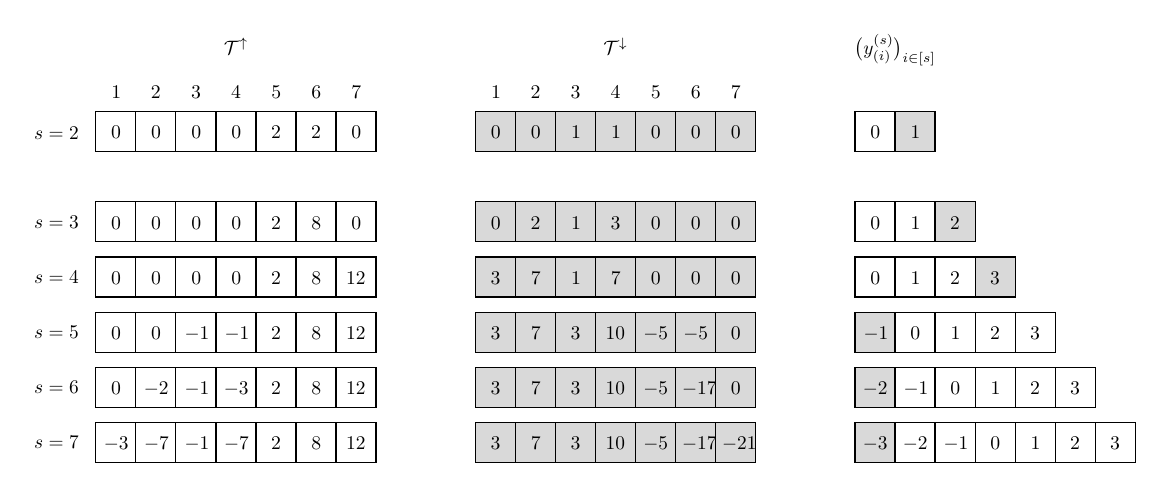
\begin{tikzpicture}[scale=0.7, every node/.style={scale=0.7},>=latex]
% https://tex.stackexchange.com/questions/228835/how-to-draw-adjacency-array-with-tikz
\matrix[mymat,anchor=west,row 2/.style={nodes=draw}]
at (0,0) 
(mat1)
{
 1 & 2 & 3 & 4 & 5 & 6 & 7\\
0 & 0 & 0 & 0 & 2 & 2 & 0 \\
};
\matrix[mymat,right=of mat1,row 2/.style={nodes={draw,fill=gray!30}}]
(mat2)
{
1 & 2 & 3 & 4 & 5 & 6 & 7 \\
0 & 0 & 1 & 1 & 0 & 0 & 0\\
};
\matrix[mymat,right=of mat2,row 2/.style={nodes=draw}]
(mat2b)
{
 & {\color{white}.}\\
0 &  |[draw,black, fill=gray!30]|1\\
};

\node[above=0pt of mat1] (titup) {$ \mathcal T^{\uparrow}$};

\node[above=0pt of mat2] (titdown) {$ \mathcal T^{\downarrow}$};

\node[above=0pt of mat2b,yshift=-0.2cm] (tit) {$ \big(y^{(s)}_{(i)}\big)_{i\in[s]}$};


\matrix[mymats=white,anchor=west]
at (0,-2) 
(mat3)
{
0 & 0 & 0 & 0 & 2 & 8 & 0 \\
};
\matrix[mymats=gray!30,right=of mat3]
(mat4)
{
0 & 2 & 1 & 3 & 0 & 0 & 0 \\
};
\matrix[mymats=white,right=of mat4]
(mat4b)
{
0 & 1 & |[draw,black, fill=gray!30]|2\\
};


\matrix[mymats=white,anchor=west]
at (0,-3) 
(mat5)
{
0 & 0 & 0 & 0 & 2 & 8 & 12 \\
};
\matrix[mymats=gray!30,right=of mat5]
(mat6)
{
3 & 7 & 1 & 7 & 0 & 0 & 0 \\
};
\matrix[mymats=white,right=of mat6]
(mat6b)
{
0 & 1 & 2 &  |[draw,black, fill=gray!30]|3\\
};

\matrix[mymats=white,anchor=west]
at (0,-4) 
(mat7)
{
0 & 0 & -1 & -1 & 2 & 8 & 12 \\
};
\matrix[mymats=gray!30,right=of mat7]
(mat8)
{
3 & 7 & 3 & 10 & -5 & -5 & 0 \\
};
\matrix[mymats=white,right=of mat8]
(mat8b)
{
 |[draw,black, fill=gray!30]|-1 & 0 & 1 & 2 & 3\\
};

\matrix[mymats=white,anchor=west]
at (0,-5) 
(mat9)
{
0 & -2 & -1 & -3 & 2 & 8 & 12 \\
};
\matrix[mymats=gray!30,right=of mat9]
(mat10)
{
3 & 7 & 3 & 10 & -5 & -17 & 0  \\
};
\matrix[mymats=white,right=of mat10]
(mat10b)
{
 |[draw,black, fill=gray!30]|-2 & -1 & 0 & 1 & 2 & 3\\
};

\matrix[mymats=white,anchor=west]
at (0,-6) 
(mat11)
{
-3 & -7 & -1 & -7 & 2 & 8 & 12 \\
};
\matrix[mymats=gray!30,right=of mat11]
(mat12)
{
3 & 7 & 3 & 10 & -5 & -17 & -21  \\
};
\matrix[mymats=white,right=of mat12]
(mat12b)
{
|[draw,black, fill=gray!30]|-3 & -2 & -1 & 0 & 1 & 2 & 3\\
};


\node[left=0pt of mat1,yshift=-0.4cm] (idx2) {$s=2$};

\node[left=0pt of mat3] (idx3) {$s=3$};
\node[left=0pt of mat5] (idx4) {$s=4$};
\node[left=0pt of mat7] (idx5) {$s=5$};
\node[left=0pt of mat9] (idx6) {$s=6$};
\node[left=0pt of mat11] (idx7) {$s=7$};


% \node[above=0pt of mat1]
%   (cella) {Cell A};
% \node[above=0pt of mat2]
%   (cellb) {Cell B};
% \node at (mat4-1-7.north|-cellb)
%   (cellx) {Cell X};

% \begin{scope}[shorten <= -2pt]
% \draw[*->]
%   (mat1-2-1.south) -- (mat3-1-1.north);
% \draw[*->]
%   (mat1-2-2.south) -- (mat3-1-3.north);
% \draw[*->]
%   (mat1-2-3.south) -- (mat3-1-4.north);
% \draw[*->]
%   (mat1-2-4.south) -- (mat3-1-7.north);
% \draw[*->]
%   (mat1-2-5.south) -- (mat3-1-9.north);

% \draw[*->]
%   (mat2-2-1.south) -- (mat4-1-1.north);
% \draw[*->]
%   (mat2-2-2.south) -- (mat4-1-3.north);
% \draw[*->]
%   (mat2-2-3.south) -- (mat4-1-4.north);
% \draw[*->]
%   (mat2-2-4.south) -- (mat4-1-6.north);

% \draw[*->,dashed,line width=0.7pt]
%   (mat4-1-1.north) to[out=90,in=-60,looseness=0.4] (mat1-2-3.south);
% \draw[*->,dashed,line width=0.7pt]
%   (mat3-1-6.north) to[out=90,in=-90] (mat2-2-1.south);
% \draw[*->,dashed,line width=0.7pt]
%   (mat4-1-7.north) ..
%     controls ++ (0.5,0.5) and ++(-1,-0.7) ..  
%   (cellx.south);
% \end{scope}
\end{tikzpicture}
\caption{Illustration on the way the two weighted-Fenwick trees $\mathcal T^{\uparrow}$ and $\mathcal T^{\downarrow}$ are updated along the iterations to compute the entropies of each prefix sequence $\textbf y^{(s)}$, $s=1,\dots , 7$.}
\label{fig:Wfenwick_tree}
\end{figure}

\end{comment}





\section{Proofs}


\subsection{Proof of Theorem~\ref{thm:indu}}
The CRPS is defined by
\[\mathrm{CRPS}(F,y) = \int_{-\infty}^{+\infty} \big( F(s) - \mathds 1_{s\geq y}\big)^2 ds.\]
The associated entropy is 
\[ \min_F \mathds E[ \mathrm{CRPS}(F,Y)].\]
Considering its empirical counterpart, the minimizer is the empirical CDF.
\[\hat F:s\mapsto \frac1n \sum_{i=1}^n \mathds 1_{s\geq y_i}.\]
We deduce that the empirical entropy is given by
\allowdisplaybreaks
\begingroup
\begin{align*}
&\frac1n \sum_{i=1}^n\mathrm{CRPS}(\widehat F,y_i)\\
& = \frac1n \sum_{i=1}^n \int_{-\infty}^{+\infty} \big( \hat F(s) - \mathds 1_{s\geq y_i}\big)^2 ds\\
&=   \frac1n \sum_{i=1}^n \int_{-\infty}^{+\infty} \big( \frac1n \sum_{j=1}^n \mathds 1_{s\geq y_j} - \mathds 1_{s\geq y_i}\big)^2 ds\\
&=   \frac{1}{n^3} \sum_{i,j,k} \int_{-\infty}^{+\infty} \big( \mathds 1_{s\geq y_j} - \mathds 1_{s\geq y_i}\big)\big( \mathds 1_{s\geq y_k} - \mathds 1_{s\geq y_i}\big)  ds\\
&=   \frac{2}{n^3} \sum_{i<j<k} \int_{-\infty}^{+\infty} \big( \mathds 1_{s\geq y_{(j)}} - \mathds 1_{s\geq y_{(i)}}\big)\big( \mathds 1_{s\geq y_{(k)}} - \mathds 1_{s\geq y_{(i)}}\big)  ds\\
&\qquad + \frac{2}{n^3} \sum_{j<i<k} \int_{-\infty}^{+\infty} \big( \mathds 1_{s\geq y_{(j)}} - \mathds 1_{s\geq y_{(i)}}\big)\big( \mathds 1_{s\geq y_{(k)}} - \mathds 1_{s\geq y_{(i)}}\big)  ds\\
&\qquad + \frac{2}{n^3} \sum_{j<k<i} \int_{-\infty}^{+\infty} \big( \mathds 1_{s\geq y_{(j)}} - \mathds 1_{s\geq y_{(i)}}\big)\big( \mathds 1_{s\geq y_{(k)}} - \mathds 1_{s\geq y_{(i)}}\big)  ds\\
&\qquad + \frac{2}{n^3} \sum_{j<i} \int_{-\infty}^{+\infty} \big( \mathds 1_{s\geq y_{(j)}} - \mathds 1_{s\geq y_{(i)}}\big)^2  ds\\
&=   \frac{2}{n^3} \sum_{i<j<k}  (y_{(j)}-y_{(i)})  \quad + 0\quad  + \frac{2}{n^3} \sum_{j<k<i}  (y_{(i)}-y_{(k)})+ \frac{2}{n^3} \sum_{j<i} (y_{(i)}-y_{(j)}) \\ 
&=   \frac{2}{n^3} \sum_{i=1}^{n-2} \sum_{j=i+1}^{n-1}  (n-j)(y_{(j)}-y_{(i)}) - \frac{2}{n^3} \sum_{j=1}^{n-2} \sum_{k=j+1}^{n-1}  \sum_{i=k+1}^{n}(y_{(k)}-y_{(i)})+\frac{2}{n^3} \sum_{i<j} (y_{(j)}-y_{(i)})\\ 
&=   \frac{2}{n^3} \sum_{i=1}^{n-1} \sum_{j=i+1}^{n}  (n-j+1)(y_{(j)}-y_{(i)}) - \frac{2}{n^3} \sum_{j=1}^{n-2} \sum_{k=j+1}^{n-1}  \sum_{i=k+1}^{n}(y_{(k)}-y_{(i)})\\ 
&=  - \frac{2}{n^3} \sum_{i=1}^{n-1} [n(n-i) -\frac{n(n-1)}{2}+\frac{i(i-1)}{2}] y_{(i)}  + \frac{2}{n^3}\sum_{j=2}^{n}(n-j+1)(j-1)y_{(j)}\\
&\qquad -\frac{2}{n^3} \sum_{i=3}^{n} \sum_{k=2}^{i-1} \sum_{j=1}^{k-1}  (y_{(k)}-y_{(i)})\\ 
&= -  \frac{2}{n^3} \sum_{i=1}^{n-1} \frac12(n-i)(n-i+1) y_{(i)}  + \frac{2}{n^3}\sum_{j=2}^{n}(n-j+1)(j-1)y_{(j)}-\frac{2}{n^3} \sum_{i=3}^{n} \sum_{k=2}^{i-1} (k-1)  (y_{(k)}-y_{(i)})\\ 
&=  - \frac{1}{n^3} \sum_{i=1}^{n-1} (n-i)(n-i+1) y_{(i)}  + \frac{2}{n^3}\sum_{j=2}^{n}(n-j+1)(j-1)y_{(j)}\\
&\qquad +\frac{2}{n^3} \sum_{i=3}^{n} \frac{(i-2)(i-1)}{2} y_{(i)} - \frac{2}{n^3} \sum_{k=2}^{n-1} (n-k)(k-1)y_{(k)} \\ 
&= -  \frac{1}{n^3} \sum_{i=1}^{n-1} (n-i)(n-i+1) y_{(i)}  +\frac{1}{n^3} \sum_{i=3}^{n} (i-2)(i-1) y_{(i)} +\frac{2}{n^3} \sum_{k=2}^{n} (k-1)y_{(k)}\\
&= -  \frac{1}{n^3} \sum_{i=1}^{n} (n-i)(n-i+1) y_{(i)}  +\frac{1}{n^3} \sum_{i=3}^{n} (i-2)(i-1) y_{(i)} +\frac{2}{n^3} \sum_{k=1}^{n} (k-1)y_{(k)}\\
&= \frac{1}{n^3} \sum_{i=1}^{n} \left[(i-2)(i-1)+2(i-1)-(n-i)(n-i+1) \right] y_{(i)}  \\
&= \frac{1}{n^3} \sum_{i=1}^{n} \left[i(i-1)-(n-i)(n-i+1) \right] y_{(i)}  \\
&=   \frac{1}{n^3} \sum_{i=1}^{n} (i-1)i (y_{(i)}-y_{(n-i+1)}) .
%&= -  \frac{1}{n^3} \sum_{i=1}^{n} (i-1)(i-2) (y_{(i)}+y_{(n-i+1)})  + \frac{2}{n^3}\sum_{j=1}^{n}(n-j)(j-1)\big(y_{(j)}+y_{(n-j+1)}\big)\\
%&=  \frac{1}{n^3} \sum_{i=1}^{n} (i-1)(2n-3i+2) (y_{(i)}+y_{(n-i+1)})
  \end{align*}
\endgroup
We denote by $\textbf y^{(n)}$ the vector of size $n$ corresponding to the $n$ first entries of the vector of observations $\textbf y$ (where we consider without loss of generality that elements in $\textbf y$ have been ordered considering the permutation sorting in increasing order $\big( x_{i,k}\big)_{i: \textbf x_i \in R_j}$ for some given node $k$ and some feature $j$). From the previous computations we have 
\[\frac1n \sum_{i=1}^n\mathrm{CRPS}(\widehat F,y_i) = \frac{1}{n^3} \left(h^{(n)}_{\uparrow} -h^{(n)}_{\downarrow} \right),\]
where \begin{align*}
h^{(n)}_{\uparrow}&:=\sum_{i=1}^{n} (i-1)iy^{(n)}_{(i)}\quad \text{and} \quad
h^{(n)}_{\downarrow}:=\sum_{i=1}^{n} (i-1)i y^{(n)}_{(n-i+1)}.
\end{align*}
In the following, we derive iterative formula for both $h^{(n)}_{\uparrow}$ and $h^{(n)}_{\downarrow}$.

\paragraph{Iterative formula for $h^{(n)}_{\uparrow}$}.

\allowdisplaybreaks
\begingroup
\begin{align*}
h^{(n+1)}_{\uparrow}-h^{(n)} _{\uparrow}&=\sum_{i=1}^{n+1} (i-1)iy^{(n+1)}_{(i)} -\sum_{i=1}^{n} (i-1)iy^{(n)}_{(i)} \\
&=\sum_{i=1}^{n+1} (i-1)i y^{(n+1)}_{(i)} -\sum_{i=1}^{r_{n+1}-1} (i-1)iy^{(n+1)}_{(i)} -\sum_{i=r_{n+1}}^{n} (i-1)i y^{(n+1)}_{(i+1)} \\
&=\sum_{i=1}^{n+1} (i-1)iy^{(n+1)}_{(i)} -\sum_{i=1}^{r_{n+1}-1} (i-1)i y^{(n+1)}_{(i)} -\sum_{i=r_{n+1}+1}^{n+1} (i-2)(i-1) y^{(n+1)}_{(i)} \\
&=(r_{n+1}-1) r_{n+1} y^{(n+1)}_{(r_{n+1})} + 2\sum_{i=r_{n+1}+1}^{n+1} (i-1) y^{(n+1)}_{(i)}\\
&=[(r_{n+1}-1) r_{n+1} - 2(r_{n+1}-1)] y^{(n+1)}_{(r_{n+1})} + 2 W^{(n+1)}\\
&-2\sum_{i=1}^{r_{n+1}-1} i y^{(n+1)}_{(i)}-2S^{(n+1)}+2\sum_{i=1}^{r_{n+1}-1}  y^{(n+1)}_{(i)}\\
&=[(r_{n+1}-1) r_{n+1} - 2(r_{n+1}-1)] y^{(n+1)}_{(r_{n+1})} + 2 W^{(n+1)}\\
&-2\sum_{i=1}^{r_{n+1}-1} i y^{(n+1)}_{(i)}-2S^{(n+1)}+2S^{(n+1)}_{r_{n+1}-1}.
\end{align*}
\endgroup


\paragraph{Iterative formula for $h^{(n)}_{\downarrow}$}.

\allowdisplaybreaks
\begingroup
\begin{align*}
h^{(n+1)}_{\downarrow}-h^{(n)}_{\downarrow} &=\sum_{i=1}^{n+1} (i-1)i y^{(n+1)}_{(n-i+2)} -\sum_{i=1}^{n} (i-1)i y^{(n)}_{(n-i+1)} \\
&=\sum_{i=1}^{n+1} (n-i+1)(n-i+2) y^{(n+1)}_{(i)} -\sum_{i=1}^{n} (n-i)(n-i+1) y^{(n)}_{(i)} \\
&=\sum_{i=1}^{n+1}  (n-i+1)(n-i+2)y^{(n+1)}_{(i)} -\sum_{i=1}^{r_{n+1}-1} (n-i)(n-i+1) y^{(n+1)}_{(i)}\\
&\quad -\sum_{i=r_{n+1}}^{n} (n-i)(n-i+1) y^{(n+1)}_{(i+1)} \\
&=\sum_{i=1}^{n+1}  (n-i+1)(n-i+2) y^{(n+1)}_{(i)} -\sum_{i=1}^{r_{n+1}-1} (n-i)(n-i+1) y^{(n+1)}_{(i)}\\
&\quad -\sum_{i=r_{n+1}+1}^{n+1} (n-i+1)(n-i+2)y^{(n+1)}_{(i)} \\
&= 2\sum_{i=1}^{r_{n+1}-1}   (n-i+1)y^{(n+1)}_{(i)} + (n-r_{n+1}+1) (n-r_{n+1}+2) y^{(n+1)}_{(r_{n+1})} \\
&= 2(n+1) S^{(n+1)}_{r_{n+1}-1}-2 \sum_{i=1}^{r_{n+1}-1} i y^{(n+1)}_{(i)} + (n-r_{n+1}+1) (n-r_{n+1}+2) y^{(n+1)}_{(r_{n+1})} .
% &= 2\sum_{i=1}^{r_{n+1}-1}   (n-i)y^{(n+1)}_{(i)} + (n-r_{n+1}+1) (n-r_{n+1}) y^{(n+1)}_{(r_{n+1})} +2\sum_{i=r_{n+1}+1}^{n+1}   (2n-2i-1)y^{(n+1)}_{(i)}\\
% &=[(n-r_{n+1}+1) (n-r_{n+1})-2(2n-2r_{n+1}-1)] y^{(n+1)}_{(r_{n+1})} -4 W^{(n+1)} + (4n-2) S^{n+1}\\
% &+2\sum_{i=1}^{r_{n+1}-1}   iy^{(n+1)}_{(i)} +(-2n+2)\sum_{i=1}^{r_{n+1}-1}   y^{(n+1)}_{(i)} 
\end{align*}
\endgroup


\paragraph{Conclusion.}
Using the previous computations, we obtain that 
\begin{align*}
h^{(n+1)}_{\uparrow}-h^{(n+1)}_{\downarrow}
&=h^{(n)}_{\uparrow}-h^{(n)}_{\downarrow}
 + n\big[2r_{n+1} -3-n\big] y^{(n+1)}_{(r_{n+1})} + 2 W^{(n+1)}-2S^{(n+1)}-2nS^{(n+1)}_{r_{n+1}-1},
\end{align*}
which ends the proof.

\subsection{Proof of Lemma~\ref{lemma:fenwick_tree}}
\label{proof:lemma:fenwick_tree}

\paragraph{Querying $S^{(s)}$ in $\mathcal O(\log n)$ time.}

Let us recall that by construction, $\mathcal F$ is at iteration $s$ a Fenwick tree for the sequence $\big( \mathrm 1_{\sigma(i)\leq s} y_{\sigma(i)}\big)_{i\in[n]}$. One can thus easily see that getting the sum of all elements in $\mathcal F$ gives $S^{(s)}=\sum_{i=1}^s y^{(s)}_{(i)}=\sum_{i=1}^s y_i $. Indeed, up to ordering of the elements, the list $\big( \mathrm 1_{\sigma(i)\leq s} y_{\sigma(i)}\big)_{i\in[n]}$ is equal to the one obtained by applying the permutation $\sigma^{-1}$ namely to $\big( \mathrm 1_{i\leq s} y_{i}\big)_{i\in[n]}$ whose sum is equal to $S^{(s)}$. Hence, querying the sum of all elements of $\mathcal F$ at iteration $s$ gives $S^{(s)}$ and this operation requires $ \mathcal O(\log n)$ time since $\mathcal F$ is a Fenwick tree.


\paragraph{Querying $S^{(s)}_{r_s-1}$ in $\mathcal O(\log n)$ time.}

Let us now prove that querying the sum of all elements in $\mathcal F$ from position $1$ to $\sigma^{-1}(s)$ at iteration $s$ is equal to $S^{(s)}_{r_s}$. This will prove that $S^{(s)}_{r_s}$ can be obtained in $\mathcal O(\log n)$ time since $\mathcal F$ is a Fenwick tree. One can then get $S^{(s)}_{r_s-1}$ using that $y^{(s)}_{(r_s)}=y_s$ and thus that
\[S^{(s)}_{r_s-1}=S^{(s)}_{r_s} -y_s.\]
Indeed, $S^{(s)}_{r_s-1}=\sum_{i=1}^{r_s-1}y^{(s)}_{(i)}$ where $r_s$ is the position of insertion of $y_s$ in the non-decreasing sorted version of the list $\mathbf y^{(s-1)}$. 

% \begin{lemma} $(y^{(s)}_{(1)}, \dots,y^{(s)}_{(r_s)})$ is, up to ordering of the elements, a sub-list of the sequence $(y_{1}, \dots, y_{s})$ meaning that the former list can be obtained from the latter by simply removing some elements (again up to the ordering). \par
% More precisely, $(y^{(s)}_{(1)}, \dots,y^{(s)}_{(r_s)})$ is equal up to ordering to $(y_k \mid k\in[s], \sigma(k)\leq \sigma(s))$.
% \label{lemma:sublemma-lem2}
% \end{lemma}
% \underline{Proof of Lemma~\ref{lemma:sublemma-lem2}}. 
\bigskip
Since $y^{(s)}_{(r_s)}=y_s$, the list $(y^{(s)}_{(1)}, \dots,y^{(s)}_{(r_s)})$ exactly corresponds to all the elements in $(y_{1}, \dots, y_{s})$ smaller than $y_s$ i.e. to the list of all $y_k$ for $k\leq s$ such that $\sigma^{-1}(k)\leq \sigma^{-1}(s)$. We deduce that
\begin{equation}\label{eq:lemma2} S^{(s)}_{r_s}=\sum_{i=1}^{r_s} y^{(s)}_{(i)} = \sum_{i=1}^s \mathrm 1_{\sigma^{-1}(i)\leq \sigma^{-1}(s)} y_i=\sum_{j\in \{ \sigma^{-1}(k) \mid k\in[s]\}} \mathrm 1_{j\leq \sigma^{-1}(s)} y_{\sigma(j)}=\sum_{j=1}^{\sigma^{-1}(s)} \mathrm 1_{\sigma(j)\leq s} y_{\sigma(j)},\end{equation}
where in the penultimate equality we made the change of variable $i=\sigma(j)$ and where in the last equality we used that 
\[ \{ \sigma^{-1}(k) \mid k\in[s], \sigma^{-1}(k)\leq \sigma^{-1}(s)\}= \{ j\mid j\in[\sigma^{-1}(s)], \sigma(j)\leq s\}.\]
Since $\mathcal F$ is at iteration $s$ a Fenwick tree for the sequence $\big( \mathrm 1_{\sigma(i)\leq s} y_{\sigma(i)}\big)_{i\in[n]}$, we deduce from Eq.\eqref{eq:lemma2} that querying the sum of elements from position 1 to $\sigma^{-1}(s)$ in $\mathcal F$ gives $S^{(s)}_{r_s}$.




As a remark, one can notice that a direct consequence of this result is that querying the sum of all elements from position 1 to $\sigma^{-1}(s+1)$ at iteration $s$ from $\mathcal F$ gives $S^{(s)}_{r_{s+1}-1}$.


\paragraph{Getting $W^{(s+1)}$ in constant time given $W^{(s)}$, $S^{(s)}$ and $S^{(s+1)}_{r_{s+1}-1}$.}


The total rank-weighted sum $W^{(s)}$ can be efficiently tracked along the iterative process using the formula
\begin{equation}\label{eq:key_update_CRPS}W^{(s+1)} = W^{(s)} +r_{s+1}y_{s+1} +\sum_{i=r_{s+1}}^s y^{(s)}_{(i)}=W^{(s)}  +r_{s+1}y_{s+1} +S^{(s)}-S^{(s)}_{r_{s+1}-1},\end{equation}
where 
\[S^{(s)}_{r_{s+1}-1} = S^{(s+1)}_{r_{s+1}-1},\]
since $r_{s+1}$ is the position of insertion of $y_{s+1}$ in the list $( y^{(s)}_{(1)}, \dots, y^{(s)}_{(s)})$. 



\section{Unbiased estimate of entropies using leave-one-out}

\label{apdx:LOO}

\subsection{LOO for PMQRT}
\label{apdx:LOO_PMQRT}

We propose using a leave-one-out method to obtain an unbiased estimate of the information gain used to build the PQRT or PMQRT. In the following, we show that such LOO estimate of the entropy associated with a pinball loss $\ell_{\tau}$ with data $\textbf y=(y_1,\dots,y_n)$ can be computed efficiently.

Let us denote by $\mathcal H_n$ the entropy of the sequence $\textbf y$ and by $\mathcal H_{n,LOO}$ the leave-one-out estimate of the entropy of $\textbf y$ for the pinball loss $\ell_{\tau}$, namely
\[\mathcal H_n = \frac{1}{n}\sum_{i=1}^n \ell_{\tau}(y_i, \hat q_{\tau}),\quad \mathcal H_{n,LOO} = \frac{1}{n}\sum_{i=1}^n \ell_{\tau}(y_i, \hat q_{\tau}^{-i}),\]
where $\hat q_{\tau}$ (resp. $\hat q_{\tau}^{-i}$) is the empirical quantile of order $\tau$ of the sequence $\textbf y$ (resp. $\textbf y^{-i}:=(y_1,\dots, y_{i-1},y_{i+1},\dots, y_n)$).

Let us consider a permutation $\sigma$ sorting the sequence $\textbf y$ by increasing order. We further denote $r_i:=\sigma^{-1}(i)$ which corresponds to the position in the sorted list of the element $y_i$. Defining $r^-:=\ceil{\tau (n-1)}$ and $r^*:=\ceil{n\tau}$, we can distinguish two possible cases:
\begin{itemize}
\item If $r^-=r^*$:
    \begin{itemize}
    \item If $r_i>r^-$:  $\ell_{\tau}(y_i, \hat q^{-i}_{\tau})=\ell_{\tau}(y_i, \hat q_{\tau}) = \tau (y_i - y_{(r^*)}).$
    \item Else: $\ell_{\tau}(y_i, \hat q^{-i}_{\tau})=(1-\tau)(y_{(r^*+1)}-y_i).$
    \end{itemize}
    Hence:
    \begin{align*}\mathcal H_{n,LOO} &= \mathcal H_n - (1-\tau) \sum_{i \mid r_i\leq r^*} (y_{(r^*)} -y_i) + (1-\tau) \sum_{i \mid r_i\leq r^*} (y_{(r^*+1)} -y_i) \\
    %&= \mathcal H_n + (1-\tau) \sum_{i \mid r_i\leq r^*} (y_{(r^*+1)} - y_{(r^*)} )\\
    &= \mathcal H_n + (1-\tau) r^* (y_{(r^*+1)} - y_{(r^*)} ).
    \end{align*}
\item Else (i.e. if $r^-+1=r^*$):
    \begin{itemize}
    \item If $r_i>r^-$:  $\ell_{\tau}(y_i, \hat q^{-i}_{\tau})=\ell_{\tau}(y_i, y_{(r^*-1)}) = \tau (y_i - y_{(r^*-1)}).$
    \item Else: $\ell_{\tau}(y_i, \hat q^{-i}_{\tau})=(1-\tau)(y_{(r^*)}-y_i).$
    \end{itemize}
     Hence:
    \begin{align*}\mathcal H_{n,LOO} &= \mathcal H_n - \tau \sum_{i \mid r_i\leq r^*} (y_i-y_{(r^*)} ) + \tau \sum_{i \mid r_i\leq r^*}  (y_i-y_{(r^*-1)} )\\
    %&= \mathcal H_n + \tau \sum_{i \mid r_i\geq r^*} (y_{(r^*)} - y_{(r^*-1)} )\\
    &= \mathcal H_n + \tau (n-r^*+1) (y_{(r^*)} - y_{(r^*-1)} ). \end{align*}
\end{itemize}


All quantities $y_{(r^*-1)}, y_{(r^*)}$ and $y_{(r^*+1)}$ can be queried in $\mathcal O(\log(n))$ time using the min-max heap structures used to train PMQRT (or PQRT). Overall, a node split using or not these LOO estimates of entropies is performed in $\mathcal O(p n \log(n))$ time where $p$ is the number of features and $n$ is the number of data points in the leaf. Therefore, no additional cost is induced by using LOO.


\medskip
Figure~\ref{fig:simu_LOO_pmqrt} illustrates on a numerical example the difference on the estimated conditional quantiles when learning PMQRTs using or not without. 


\begin{figure*}[!ht]
    \centering
    \begin{subfigure}[t]{0.5\textwidth}
        \centering
        \includegraphics[height=2.2in]{pmqrt_withLOO.png}
        \caption{With LOO.}
    \end{subfigure}%
    ~ 
    \begin{subfigure}[t]{0.5\textwidth}
        \centering
        \includegraphics[height=2.2in]{pmqrt_noLOO.png}
        \caption{Without LOO.}
    \end{subfigure}
    \caption{Estimation of the conditional CDF of y given x with PMQRF with $100$ on a sample of size $n=600$ simulated from the distribution in Eq.\eqref{eq:simu_gamma}. The true conditional CDFs (smooth dashed lines) are compared to the quantile estimates obtained from PMQRF (dots).}
    \label{fig:simu_LOO_pmqrt}
\end{figure*}





\subsection{LOO for CRPS-RT}
It is noteworthy that using leave-one-out to obtain an unbiased estimate of the information gain at each node for determining the best split is very simple. In fact, the computations presented below show that the leave-one-out estimate of the information gain can be efficiently derived by appropriately scaling the standard empirical entropies.

Denoting by $\hat F^{-i}$ the empirical CDF obtained from the sequence $(y_1,\dots,y_{i-1},y_{i+1},\dots,y_n)$, we have
\allowdisplaybreaks
\begingroup
\begin{align*}
&\frac1n \sum_{i=1}^n\mathrm{CRPS}(\widehat F^{-i},y_i)\\
& = \frac1n \sum_{i=1}^n \int_{-\infty}^{+\infty} \big( \hat F^{-i}(s) - \mathds 1_{s\geq y_i}\big)^2 ds\\
&=   \frac1n \sum_{i=1}^n \int_{-\infty}^{+\infty} \big( \frac{1}{n-1} \sum_{j\neq i} \mathds 1_{s\geq y_j} - \mathds 1_{s\geq y_i}\big)^2 ds\\
&=   \frac{1}{n(n-1)^2} \sum_{i=1}^n \sum_{j\neq i} \sum_{k\neq i}\int_{-\infty}^{+\infty} \big( \mathds 1_{s\geq y_j} - \mathds 1_{s\geq y_i}\big)\big( \mathds 1_{s\geq y_k} - \mathds 1_{s\geq y_i}\big)  ds\\
&=   \frac{1}{n(n-1)^2} \sum_{i=1}^n \sum_{j=1}^n  \sum_{k=1}^n\int_{-\infty}^{+\infty} \big( \mathds 1_{s\geq y_j} - \mathds 1_{s\geq y_i}\big)\big( \mathds 1_{s\geq y_k} - \mathds 1_{s\geq y_i}\big)  ds\\
&= \frac{n^2}{(n-1)^2} \left(\frac1n \sum_{i=1}^n\mathrm{CRPS}(\widehat F,y_i) \right).
  \end{align*}
\endgroup


\bibliography{main}



\end{document}
